\section{Introduzione}
Lo scopo di questo progetto consiste nella classificazione dell'attività fisica svolta da un individuo grazie a delle misure ottenute con la board Arduino Nano 33 BLE Sense posizionata sopra la caviglia del soggetto. Dopo essersi connessi alla board tramite BLE, e a seconda del firmware caricato sull'Arduino, è possibile utilizzare l'applicazione in due modalità:
\begin{itemize}
	\item modalità acquisizione dati: l'applicazione riceve e salva i dati inviati dalla piattaforma;
	\item modalità activity tracker: l'applicazione visualizza la predizione dell'attività che il soggetto sta svolgendo (camminata, cyclette, salto con la corda oppure l'individuo è fermo).
\end{itemize}
Per questo progetto sono stati utilizzati i seguenti sensori presenti sulla board:
\begin{itemize}
	\item accelerometro triassiale; 
	\item giroscopio triassiale;
	\item sensore di temperatura e di umidità.
\end{itemize}
Tuttavia, i dati di temperatura e umidità non sono stati utilizzati poiché i dati ricavati non si sono mostrati essere significativi per l'obiettivo di questo progetto. Inoltre, è stato necessario modificare la libreria che gestisce la comunicazione con la IMU presente sul BLE\todo{presente sul modulo volevi dire? Non è sul BLE la imu o sbaglio?} (file \texttt{LSM9DS1.cpp}) per cambiare il fondo scala dell'accelerometro (che di default è impostato a 4g):
\begin{itemize}
	\item accelerometro: fondo scala 8g, frequenza di campionamento \SI{119}{\hertz};
	\item giroscopio: fondo scala 2000 dps, frequenza di campionamento \SI{119}{\hertz}.
\end{itemize}

Per l'attività di classificazione dell'attività si è scelto di utilizzare un approccio \textit{black-box}, utilizzando una rete neurale opportunamente allenata con i dati raccolti dalla board. La rete neurale, sviluppata tramite il framework Edge Impulse, è stata poi installata sull'Arduino. Utilizzando quindi un modello di \textit{edge computing}, è stato possibile realizzare un'applicazione, sviluppata grazie al framework Qt, che si occupa solamente della visualizzazione dei dati e della predizione dell'attività svolta\todo{riguardare la seconda parte se troviamo un modo migliore di dirlo, sembra che l'app si occupa della predizione ad una prima lettura. Magri "e dell'attività svolta predetta dalla rete neurale presente sulla board"}. In questo modo, si è potuto mantenere una frequenza di campionamento dei dati relativamente alta (circa \SI{66}{\hertz}) senza sovraccaricare la comunicazione BLE.
\todo{se riesco questo weekend misuro la corrente assorbita con un tester}
\section{Acquisizione dei dati}
\begin{figure}[tbh]
	\centering
	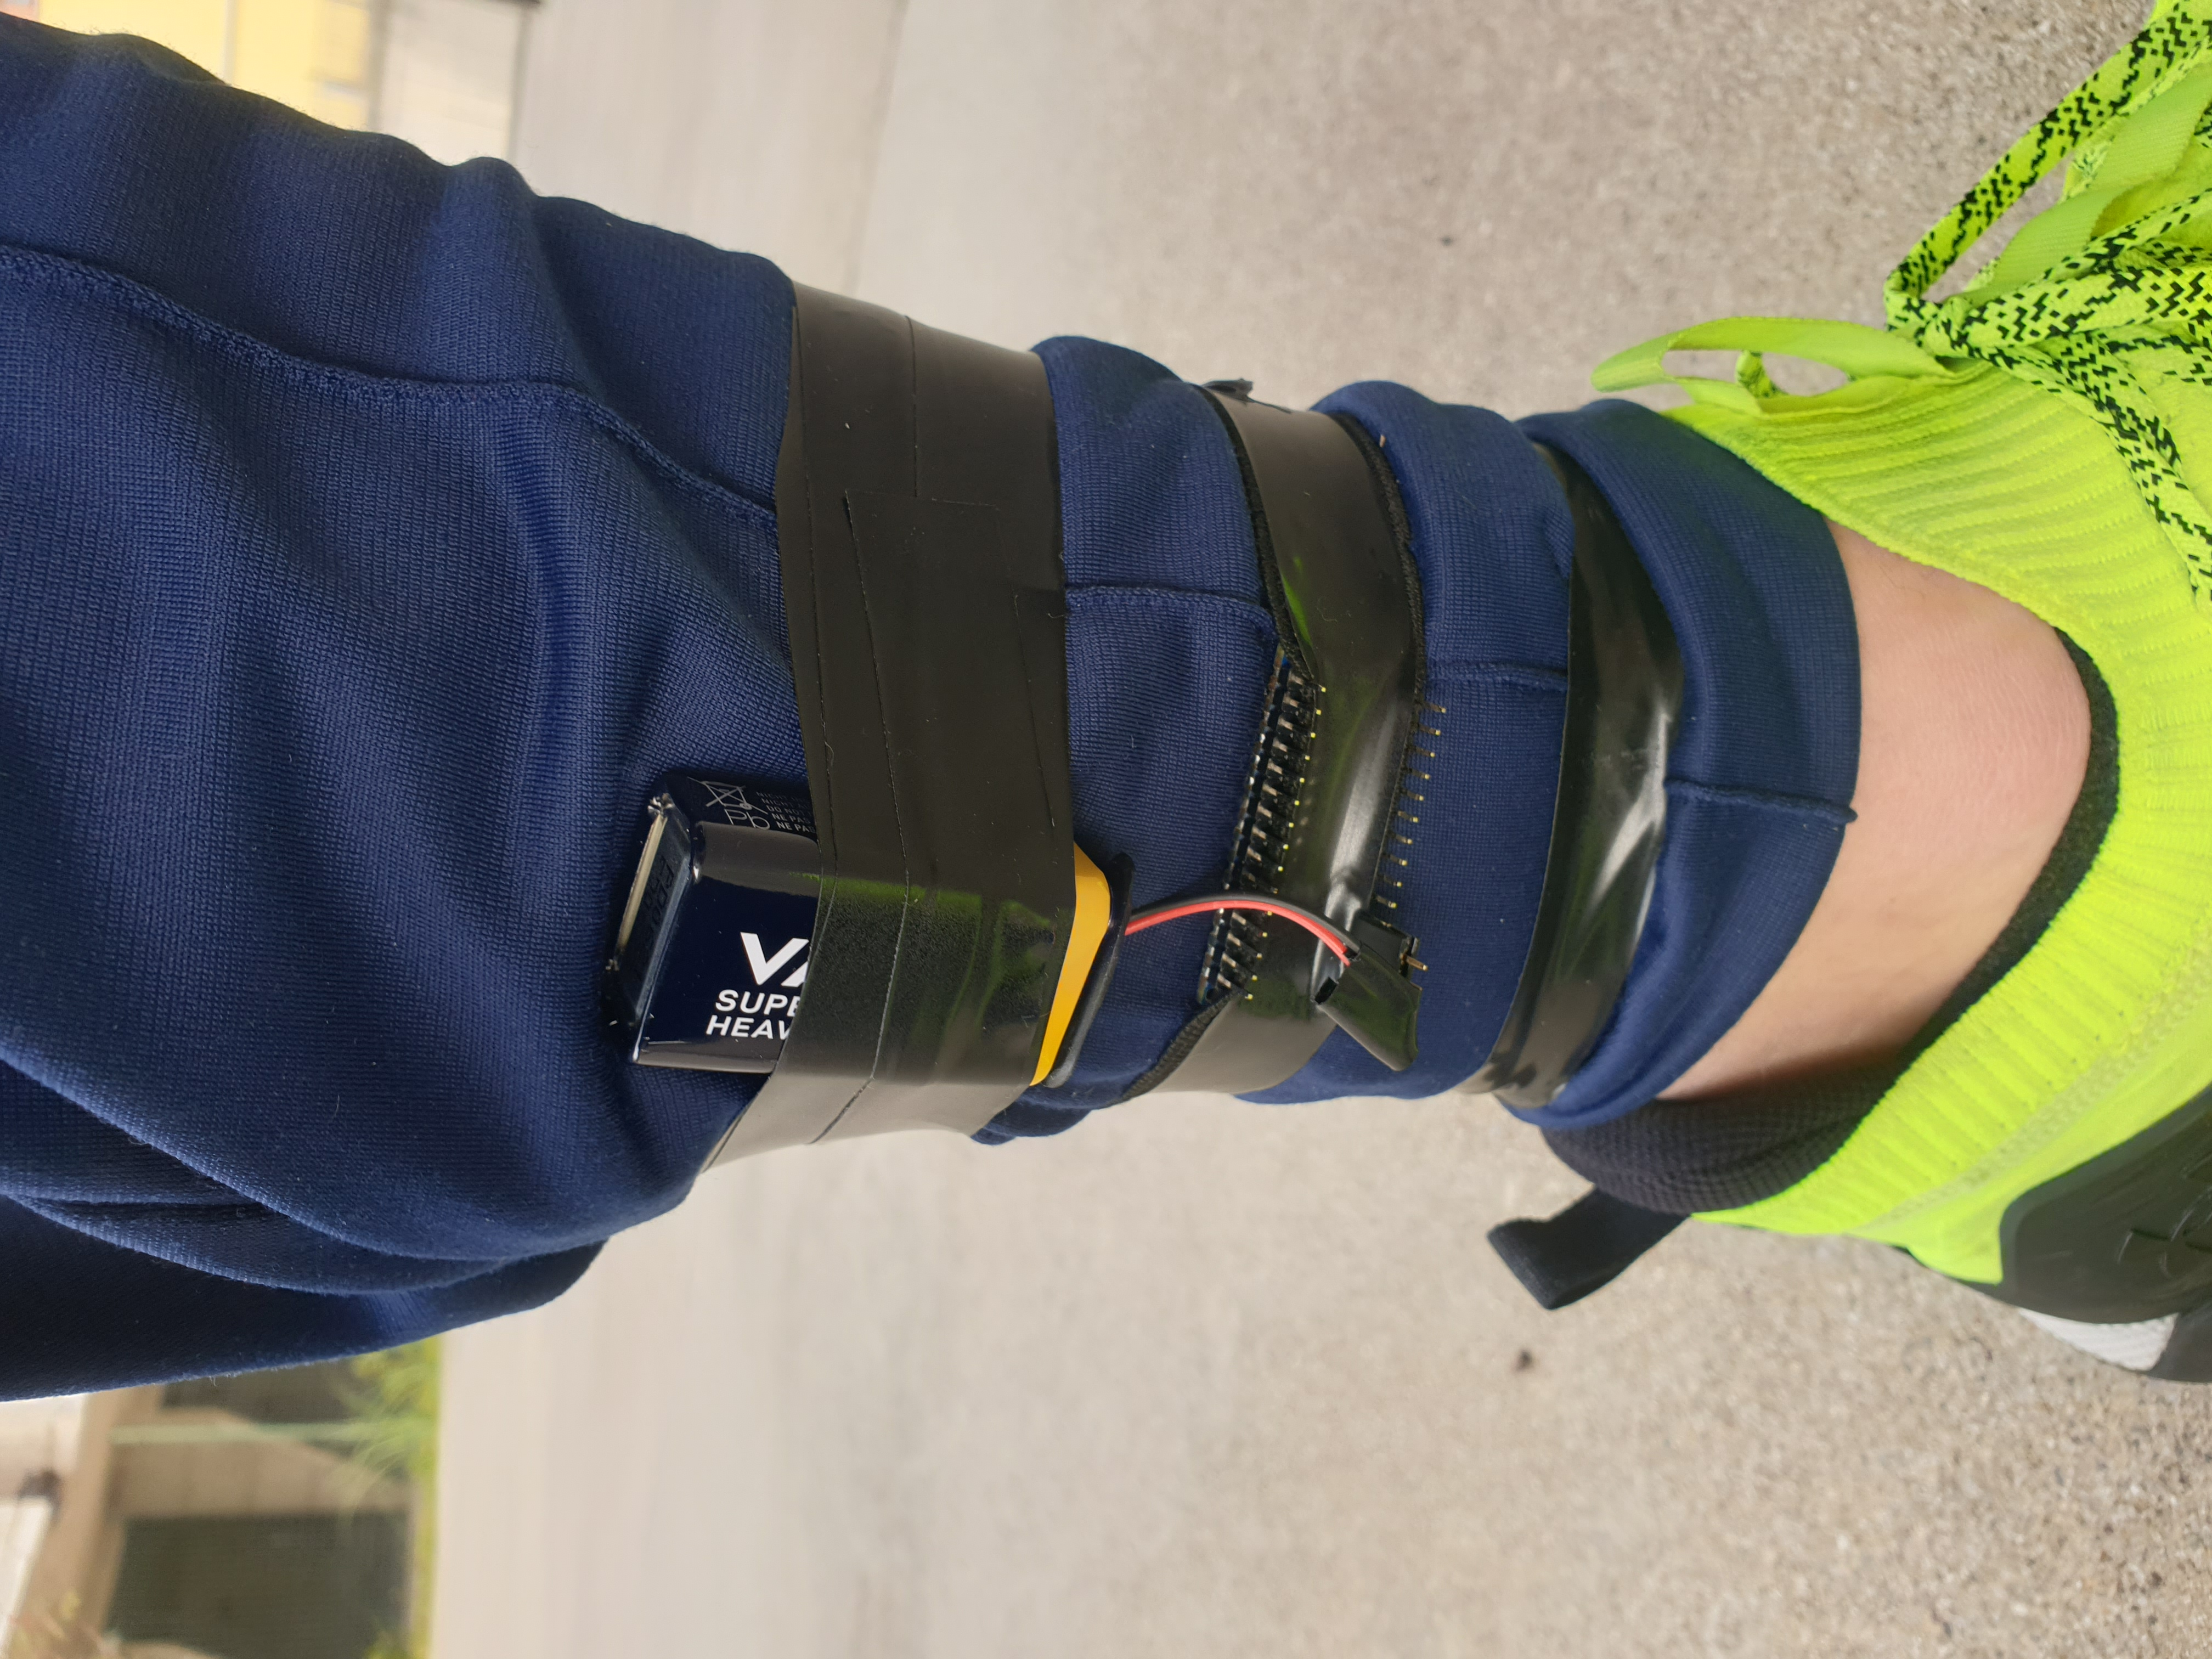
\includegraphics[angle=-90, width=0.5\linewidth]{./ImageFiles/arduino_su_gamba.jpg}
	\caption{Arduino posizionato sulla gamba del soggetto con sistema di riferimento.}
	\label{fig:arduino_su_gamba}
\end{figure}
\todo{inserire sistema di riferimento sull'immagine}
\todo{inserire foto schermata di acquisizione}
Per poter acquisire i dati con Arduino, è stato necessario sviluppare un firmware apposito che consentisse di inviare le acquisizioni utilizzando la tecnologia Bluetooth Low Energy (BLE), in cui l'Arduino è stato utilizzato nel ruolo di \textit{peripheral} mentre l'applicazione assume il ruolo di \textit{central}. La board di Arduino espone un servizio con una caratteristica su cui vengono scritti i dati delle misure. Il central viene notificato ogni volta che il \textit{peripheral} aggiorna la caratteristica e ne legge il contenuto salvandolo in un file .csv che contiene le seguenti colonne: \textit{acc x}, \textit{acc y}, \textit{acc z}, \textit{gyro x}, \textit{gyro y}, \textit{gyro z}, \textit{temp}, \textit{humidity} e \textit{timestamp}. Sull'applicazione è possibile visualizzare i dati ricevuti in real time selezionando quali canali mostrare sul grafico (figura \ref{label}).

\begin{figure}[h]
	\centering
	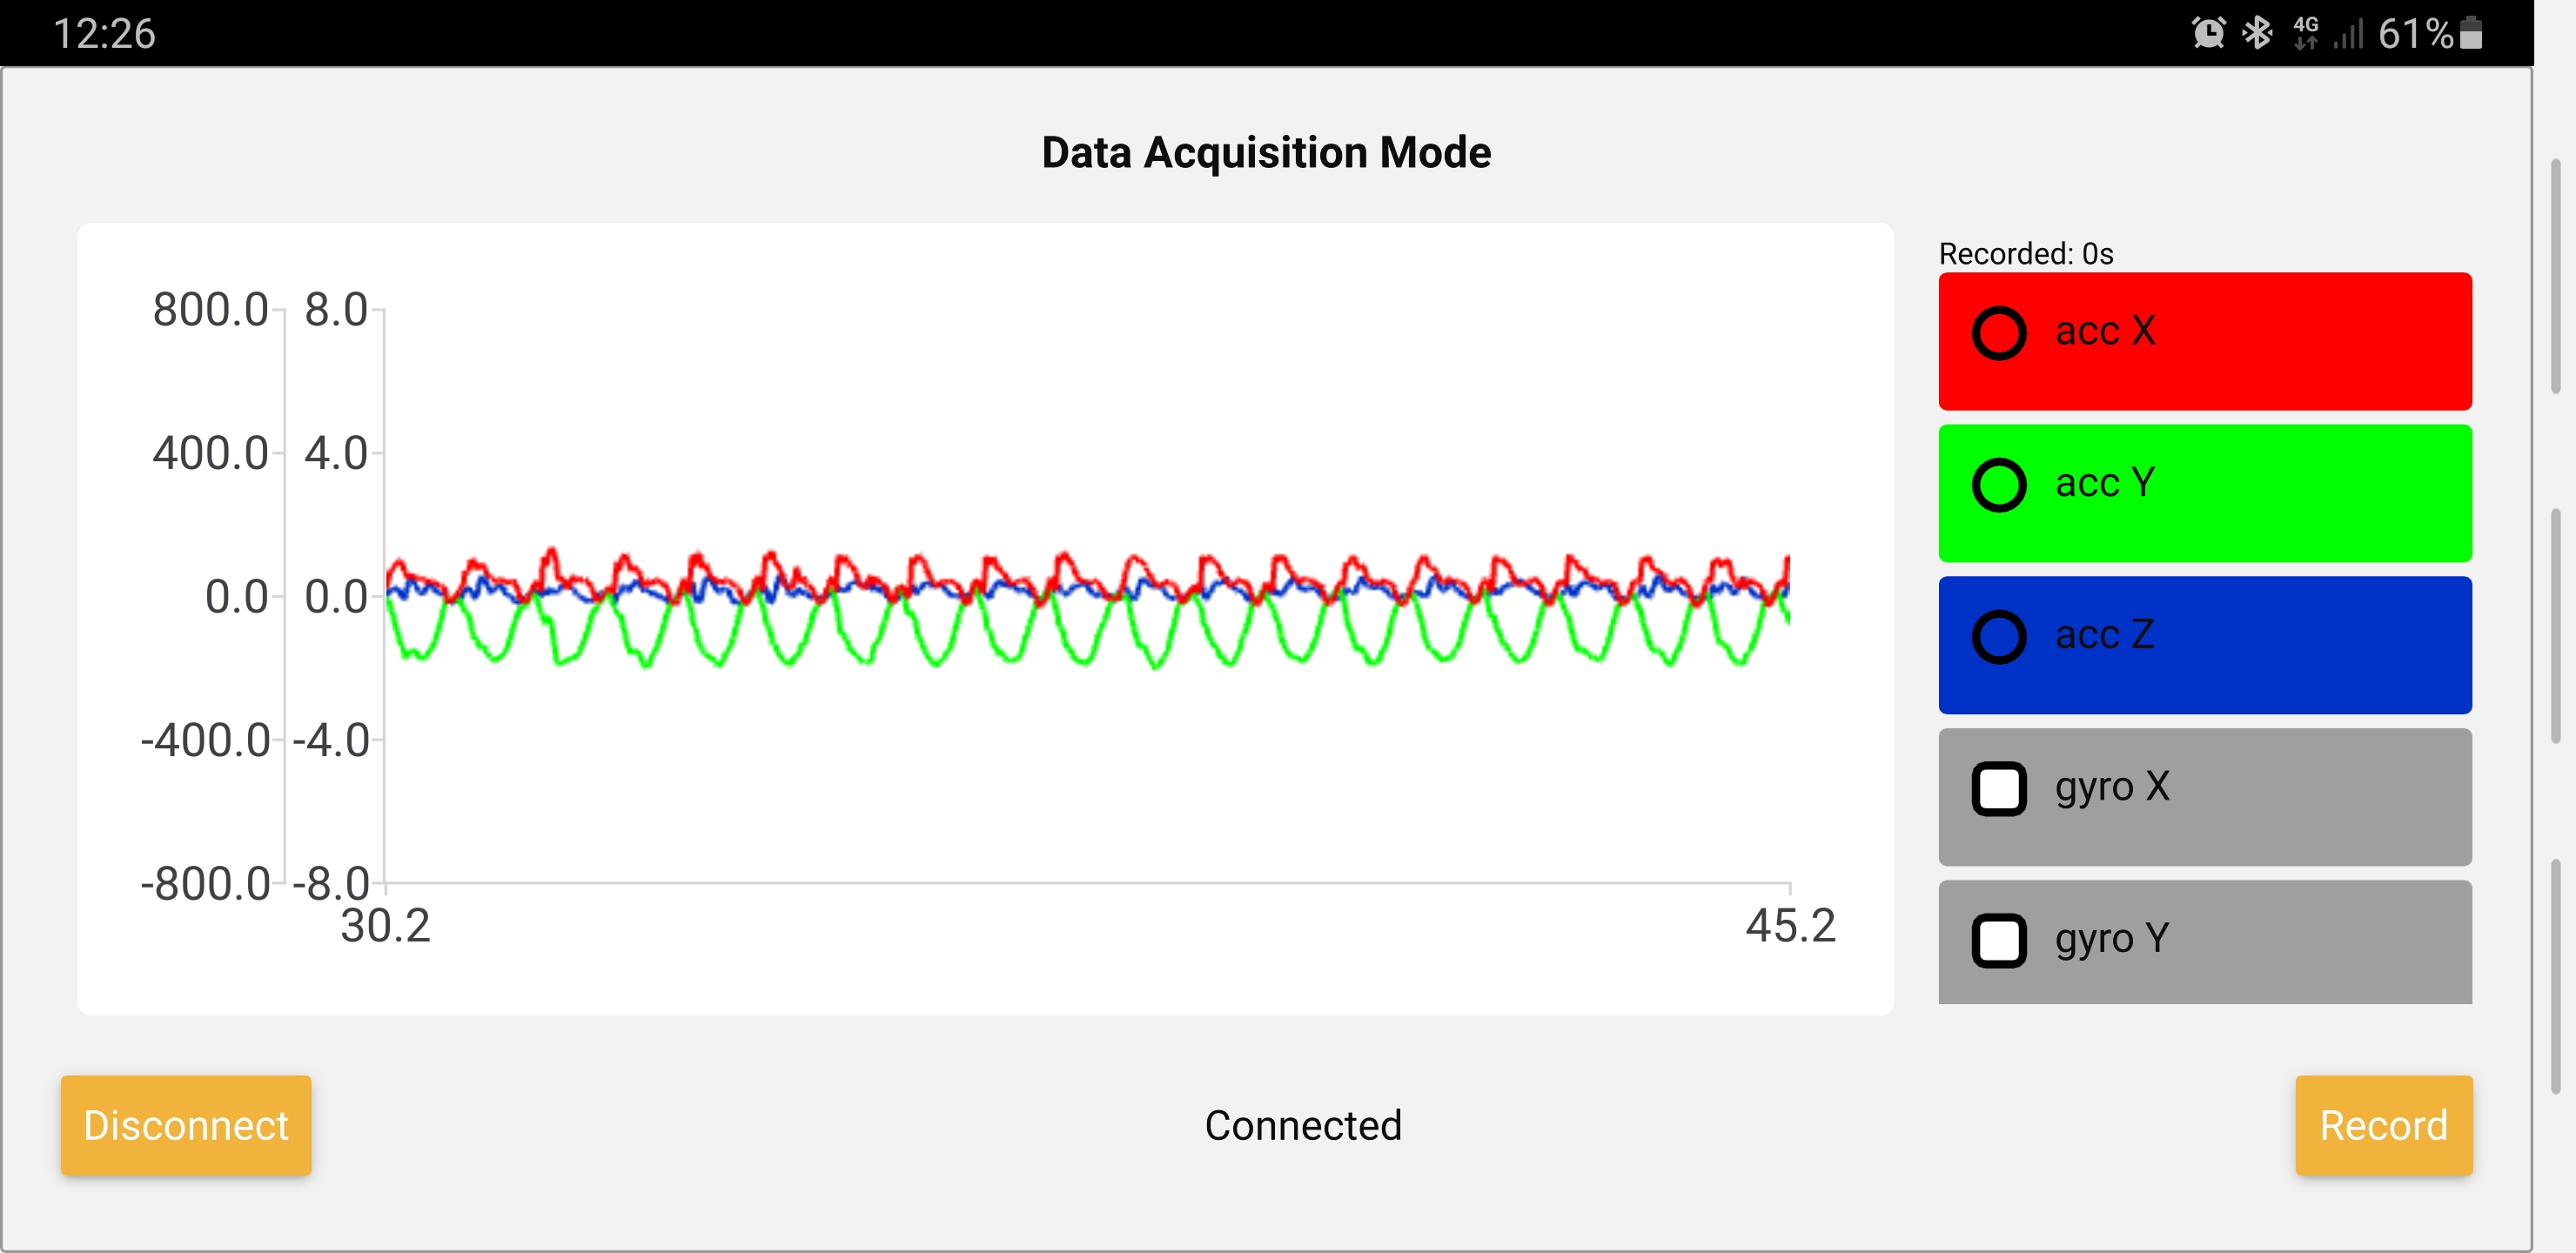
\includegraphics[width=0.49\linewidth]{./ImageFiles/acquisition_acc.jpg}
	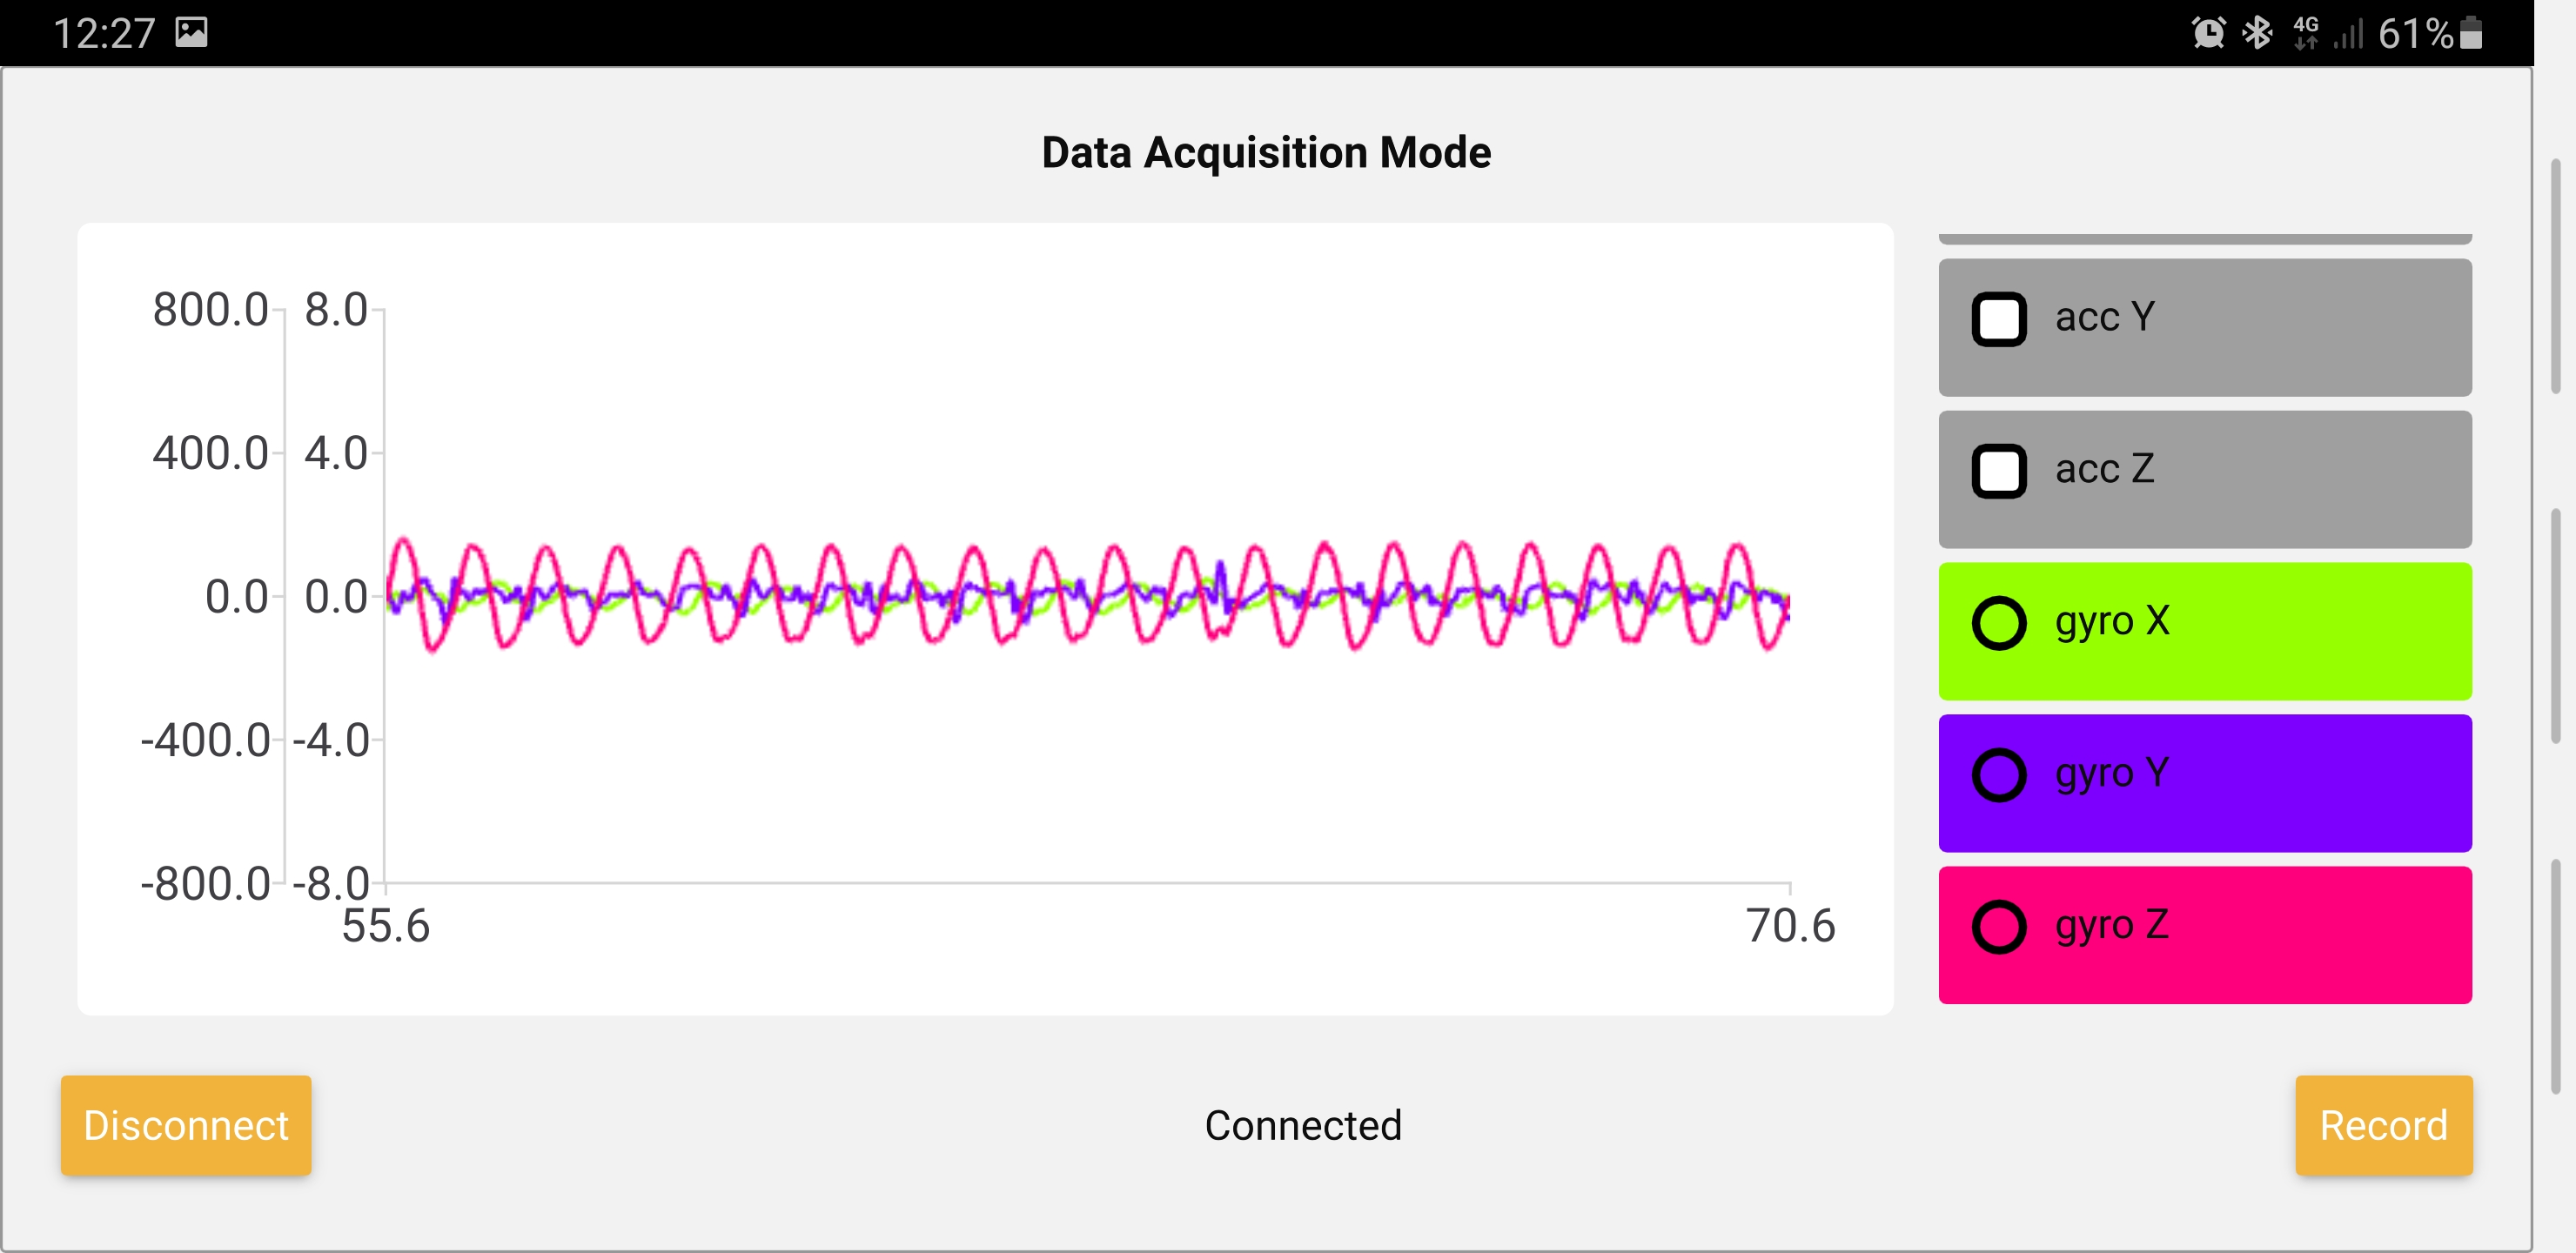
\includegraphics[width=0.49\linewidth]{./ImageFiles/acquisition_gyro.jpg}
	\caption{Schermata di acquisizione dati dell'applicazione: l'immagine a sinistra mostra i segnali dell'accelerometro mentre quella a destra mostra i segnali del giroscopio durante l'attività cyclette.}
	\label{fig:schermata_acq}
\end{figure}


Inizialmente, si è cercato di utilizzare una frequenza di campionamento dei dati pari a \SI{100}{\hertz}. Tuttavia, si è verificato che il flusso di dati non era sostenibile dal BLE. Tramite delle prove si è poi stabilito che una frequenza di campionamento dei dati sostenibile era di circa \SI{66}{\hertz} (un campione ogni \SI{15}{\milli\second}). Per assicurare una buona precisione nella frequenza di campionamento, si è scelto di utilizzare il meccanismo degli interrupt (Interrupt Service Routine), in cui un funzione di callback viene chiamata ogni \SI{15}{\milli\second}. Infatti, non è possibile utilizzare la funzione \textit{delay}, che non garantisce intervalli regolari di acquisizione. Inoltre, ciò permette di realizzare un'applicazione \textit{pseudo} concorrente, in cui la funzione \textit{loop} principale si occupa dell'invio dei dati tramite BLE, mentre un'altra funzione, attivata da un interrupt, si occupa di acquisire i dati. Ciò però non si è mostrato sufficiente a garantire una frequenza di campionamento accurata in quanto si è visto che il tempo necessario all'invio dei dati tramite BLE non è costante e portava alla perdita di alcuni dati.
Per questo motivo, è stato introdotto un buffer circolare tramite la libreria \url{https://github.com/rlogiacco/CircularBuffer}. In questo modo, se la comunicazione subisce un ritardo non si ha perdita di dati. Di seguito si riporta un esempio dei dati dell'accelerometro e giroscopio ottenuti durante una camminata di un soggetto (\Fig\ref{fig:imu_data}).
\begin{figure}[tbh]
	\centering
	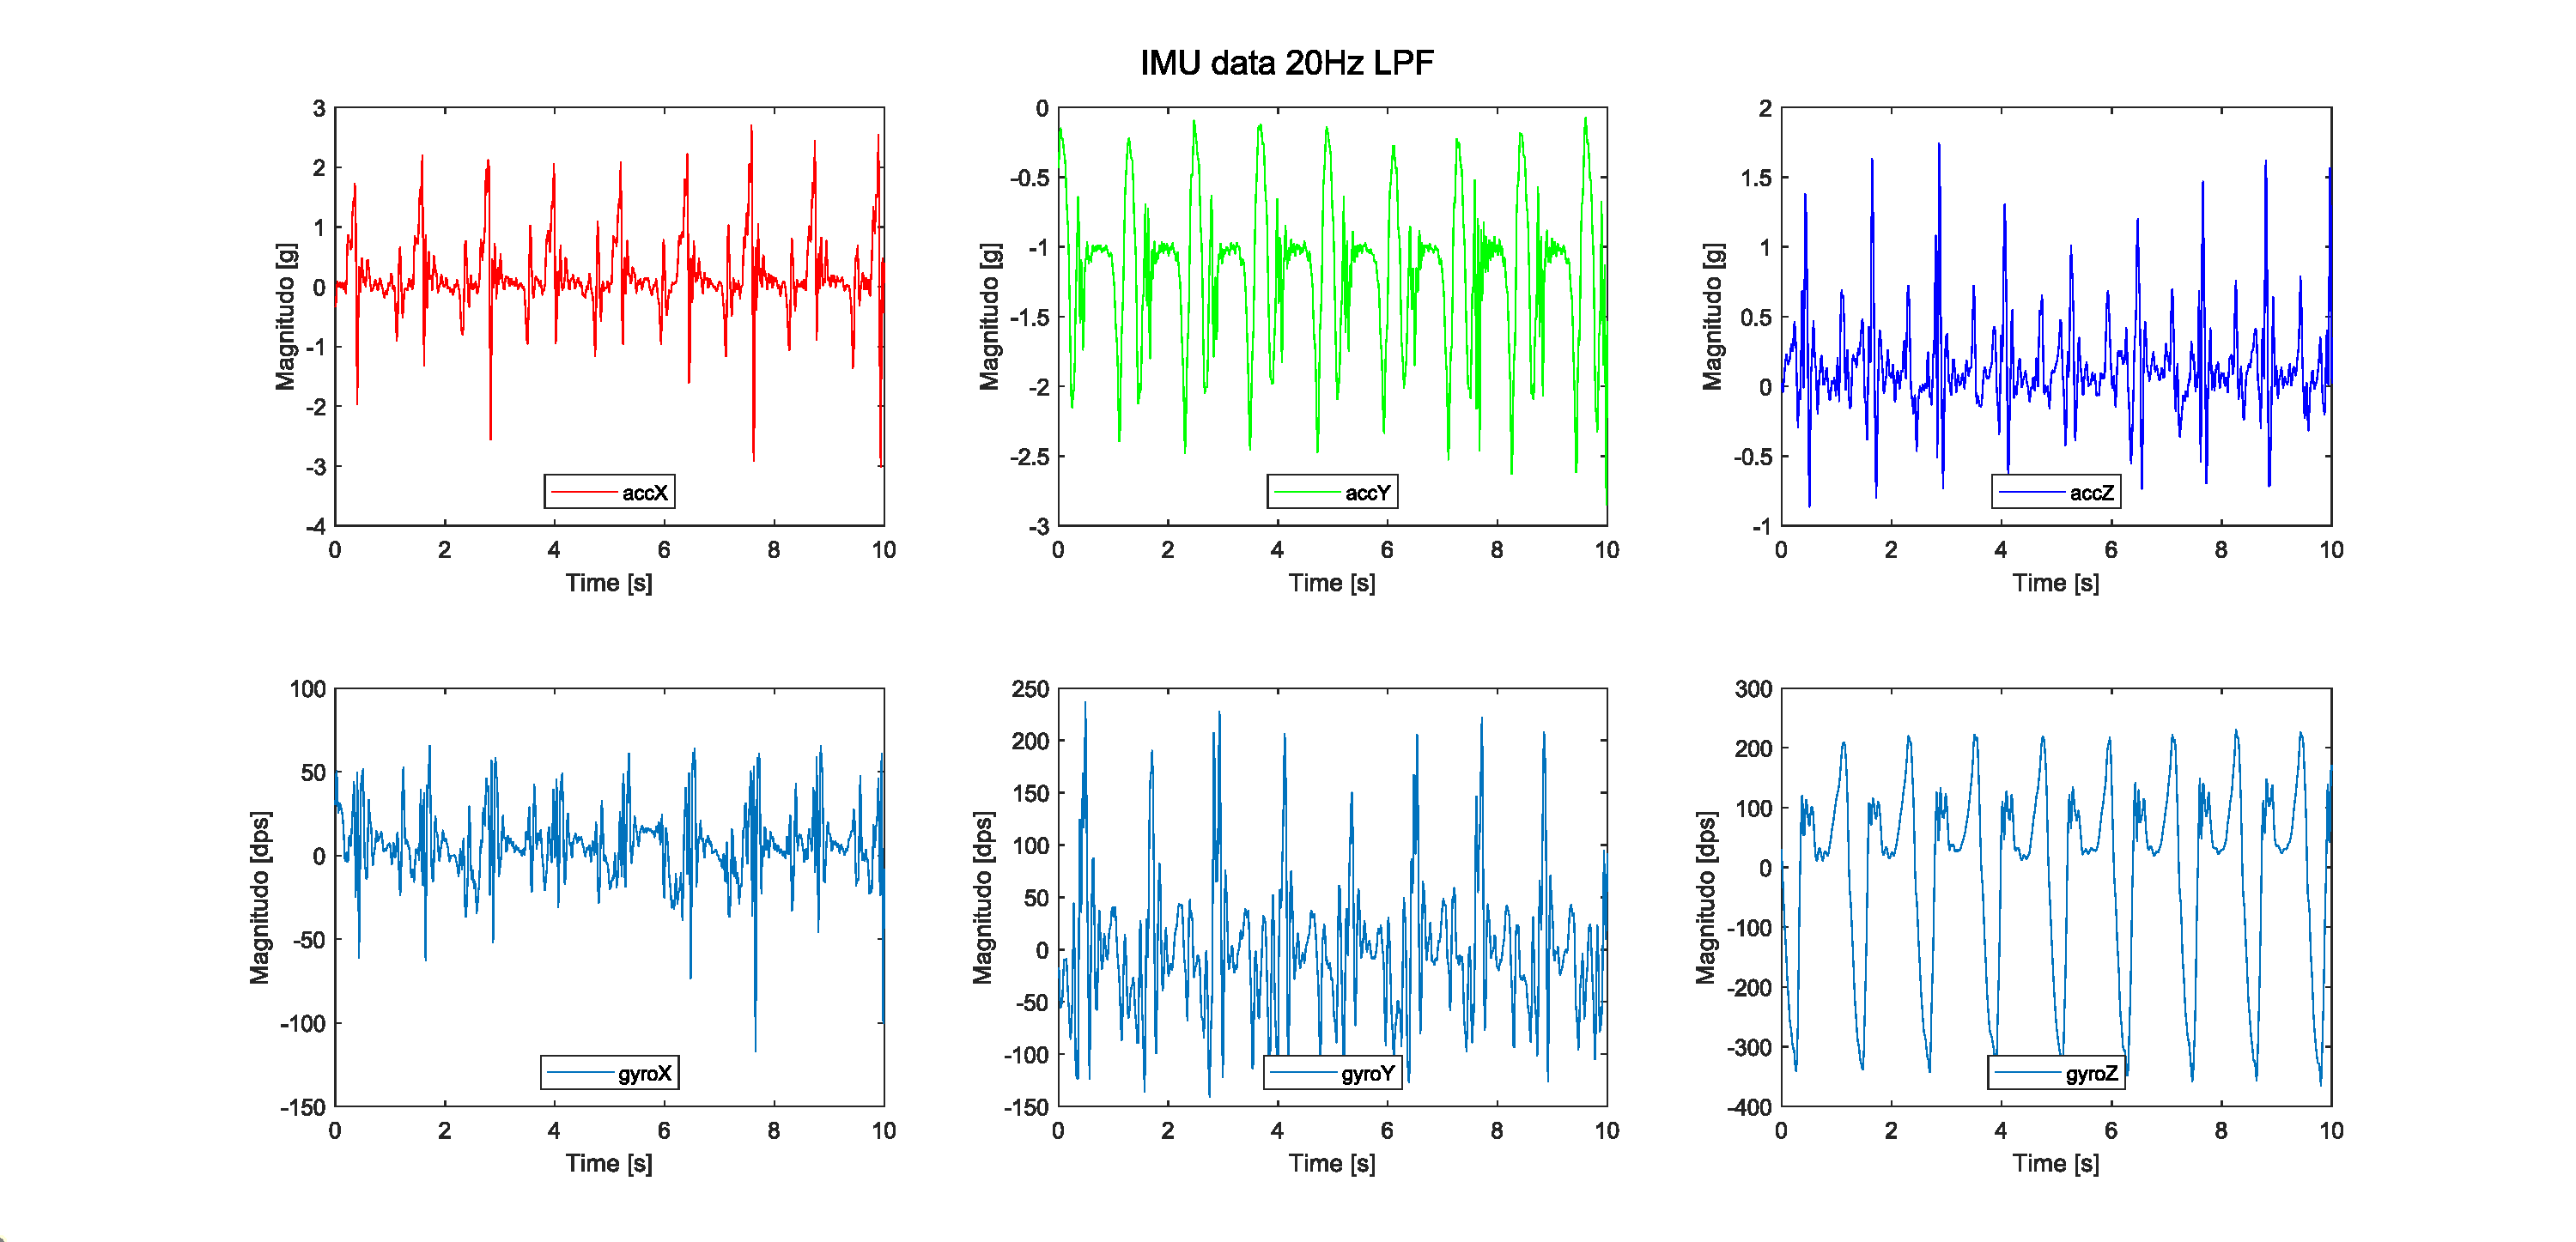
\includegraphics[width=1\linewidth]{./ImageFiles/IMU_data_example.pdf}
	\caption{Dati acquisiti dall'accelerometro e giroscopio durante una camminata. I dati sono campionati ogni \SI{15}{\milli\second} e sono stati filtrati con un filtro passa basso con frequenza di taglio di \SI{20}{\hertz}.}
	\label{fig:imu_data}
\end{figure}
Nella figura \ref{fig:time_interval}a) sono rappresentati gli intervalli di tempo tra due acquisizioni successive su una misura di \SI{76}{\second}. Il tempo medio risultante è di \SI{15.0057}{\milli\second} con una deviazione standard di \SI{0.4405}{\milli\second}. Senza buffer circolare (\Fig\ref{fig:time_interval}b)) si ottiene una media di circa \SI{16.1630}{\milli\second} con una deviazione standard di \SI{6}{\milli\second}. Infatti, è possibile vedere nell'immagine che si hanno molti più outliner.
Si tenga in considerazione che l'istante di tempo in cui si eseguiva l'acquisizione è stato misurato con la funzione \textit{millis()}, che ha errore di $\pm \SI{1}{\milli\second}$. 
\begin{figure}[tbh]
	\centering
	a)
	\begin{minipage}{.900\textwidth}
		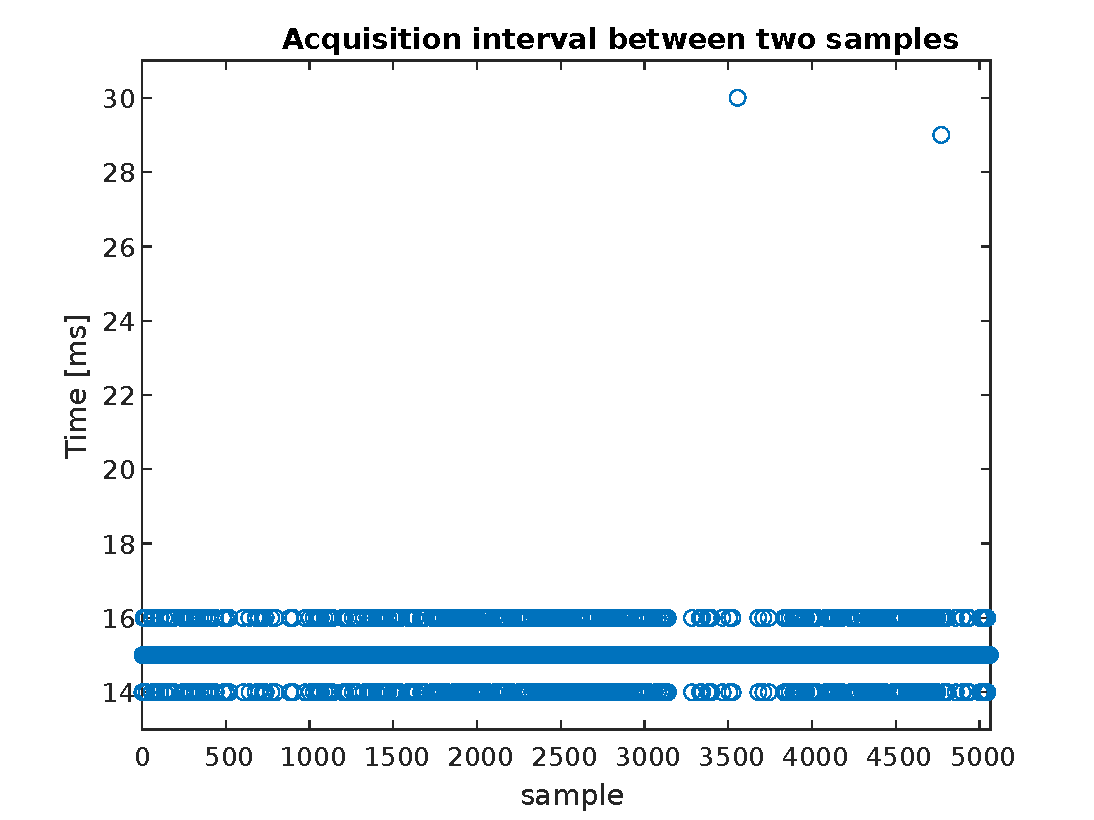
\includegraphics[width=0.8\linewidth]{./ImageFiles/interval_time.pdf}
	\end{minipage}
	\\b)
	\begin{minipage}{.900\textwidth}
		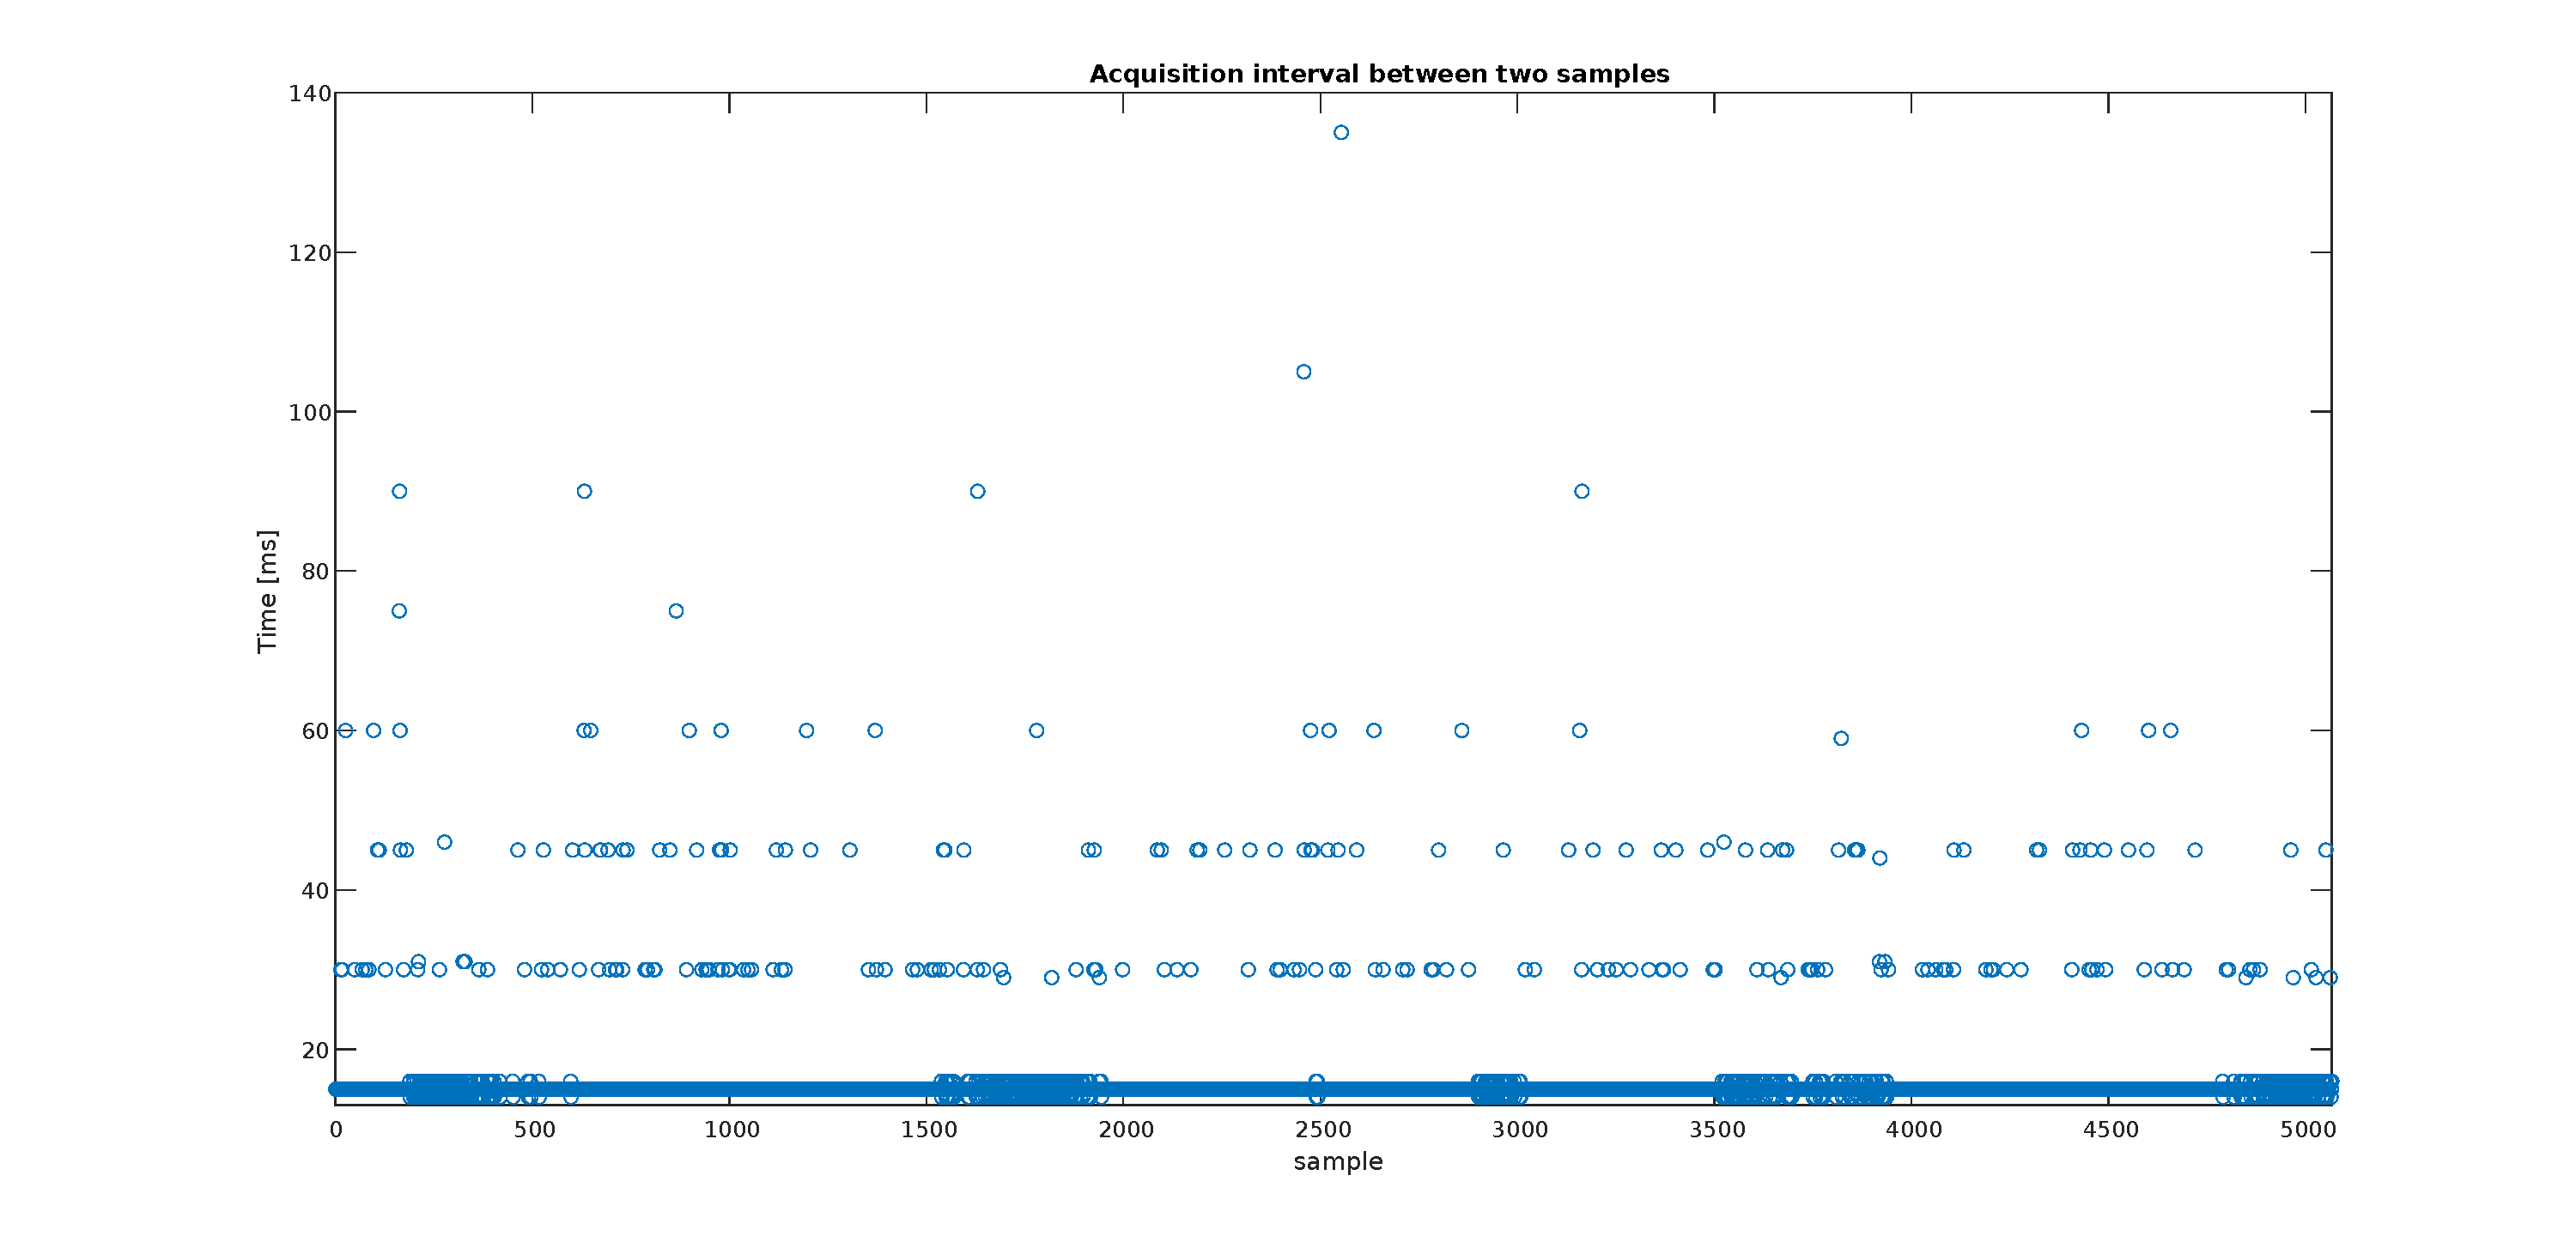
\includegraphics[width=\linewidth]{./ImageFiles/interval_time_2}
	\end{minipage}
	\caption{Tempo tra due campioni successivi su un'acquisizione di \SI{76}{\second}: a) con buffer circolare, b) senza buffer circolare.}
	\label{fig:time_interval}
\end{figure}

\section{Classificazione delle attività} \label{classifSect}
Come si può notare dalla figura \ref{fig:imu_data}, i grafici più espressivi sono quelli riguardanti l'asse z. Questo è dovuto al fatto che, per la posizione in cui si trova Arduino sulla gamba dell'individuo, l'asse z corrisponde alla direzione lungo la quale è possibile rilevare ad esempio i singoli passi effettuati durante la camminata. Considerando l'accelerometro, i singoli passi corrispondono ai picchi presenti nel segnale rappresentato.
Successivamente per realizzare la classificazione dei dati acquisiti dai sensori di Arduino e poi per visualizzarne la previsione sull'applicazione è stato sviluppato un ulteriore firmware, al cui interno sono stati creati 3 thread differenti che verranno analizzati più in dettaglio nella sezione \ref{arduinoSect}. Inoltre nel firmware sono stati gestiti anche due eventi che si possono verificare: uno si verifica quando il dispositivo si collega al BLE e quindi si riesce a scrivere il valore della predizione nella sua apposita caratteristica, mentre l'altro avviene quando il dispositivo risulta scollegato dal BLE e di conseguenza viene svuotato il buffer circolare.
In generale il funzionamento del firmware prevede che inizialmente si riempie il buffer con i dati provenienti dai sensori, poi questi dati vengono trasformati in un segnale\todo{tramire il DSP il buffer viene trasformato in un elenco di feature che vengono passate al classificatore} tramite Digital Signal Processing (DSP) che viene poi passato al classificatore realizzato su Edge Impulse per fare inferenza.
\todo{Come è stato creato l'impulse. Su cosa lavora. Cosa produce Edge Impulse. Come son state modificate le finestre. Feature spettrali. Bontà del modello e testing.}
Infine il risultato della classificazione, ovvero la previsione, viene trasmesso in una caratteristica del BLE all'applicazione, che a sua volta mostra a video l'immagine relativa all'attività fisica rilevata. Le schermate che possono essere visualizzate sull'applicazione si distinguono in base all'attività fisica rilevata come mostrato nella figura \ref{fig:attivitafisica}.
\begin{figure}[tbh]
	\centering
	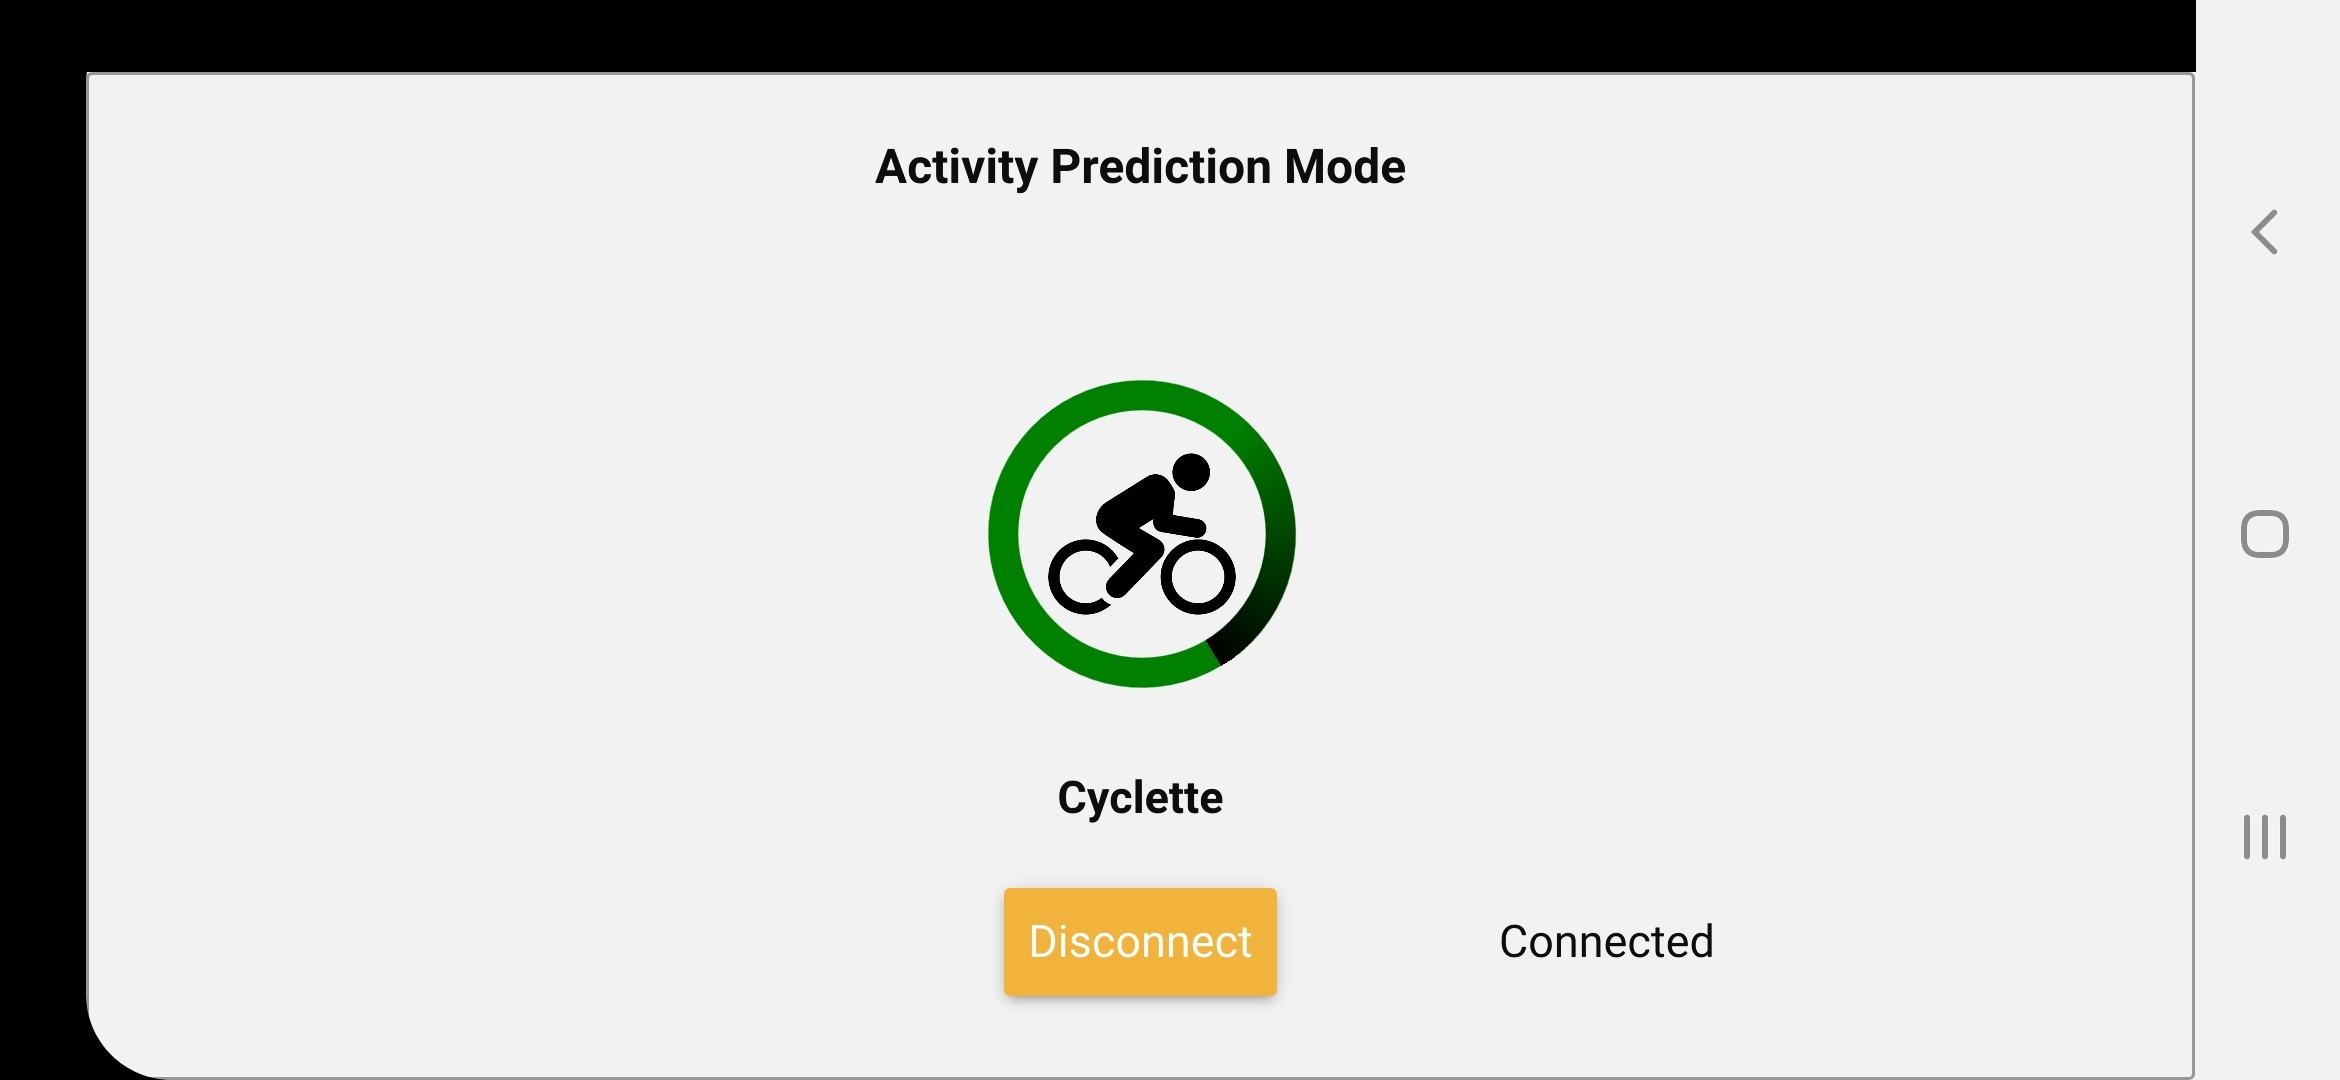
\includegraphics[width=0.4\linewidth]{./ImageFiles/cyclette}
	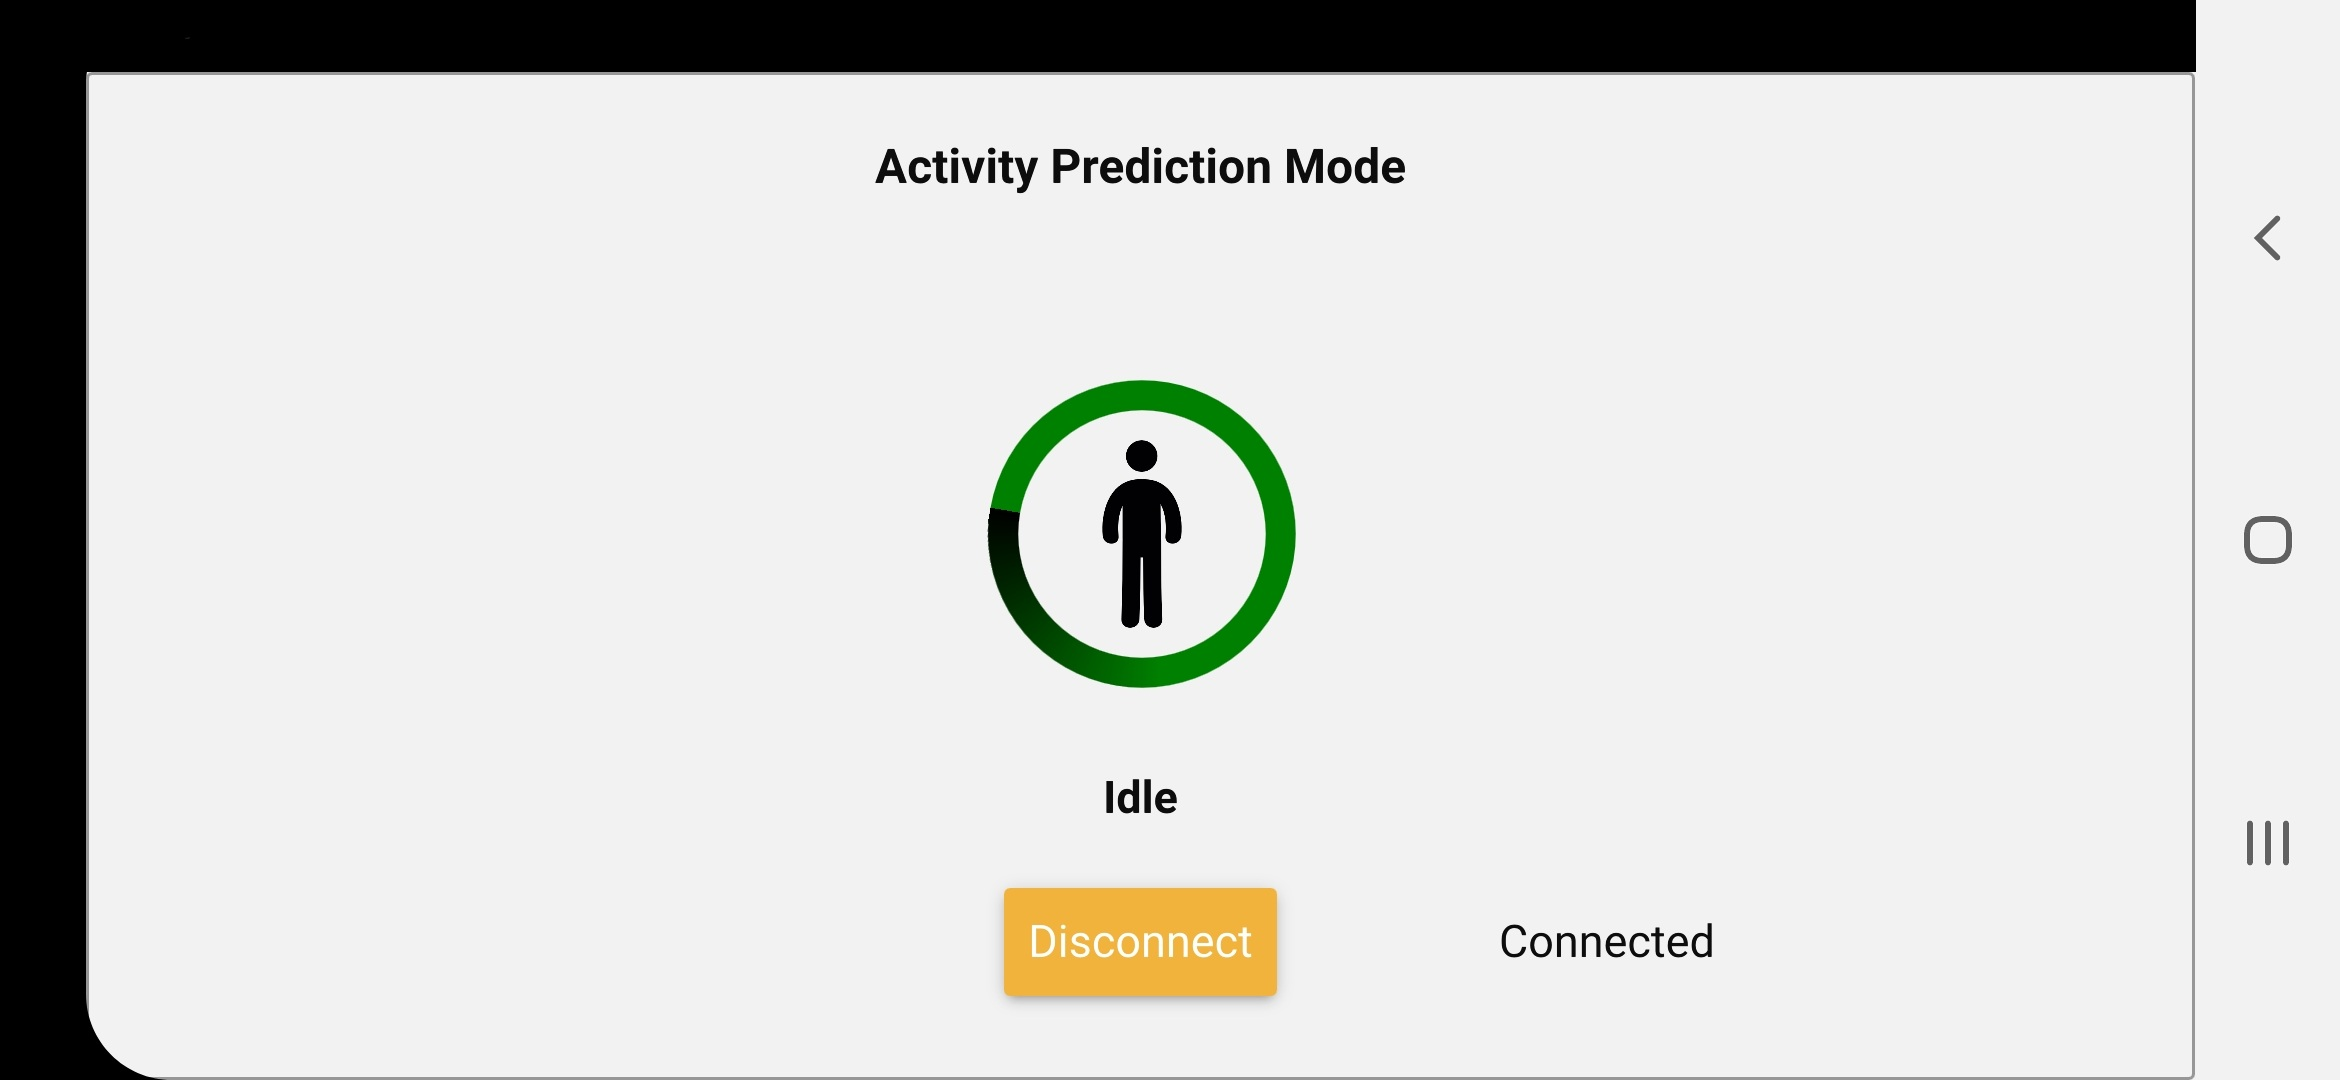
\includegraphics[width=0.4\linewidth]{./ImageFiles/idle}
	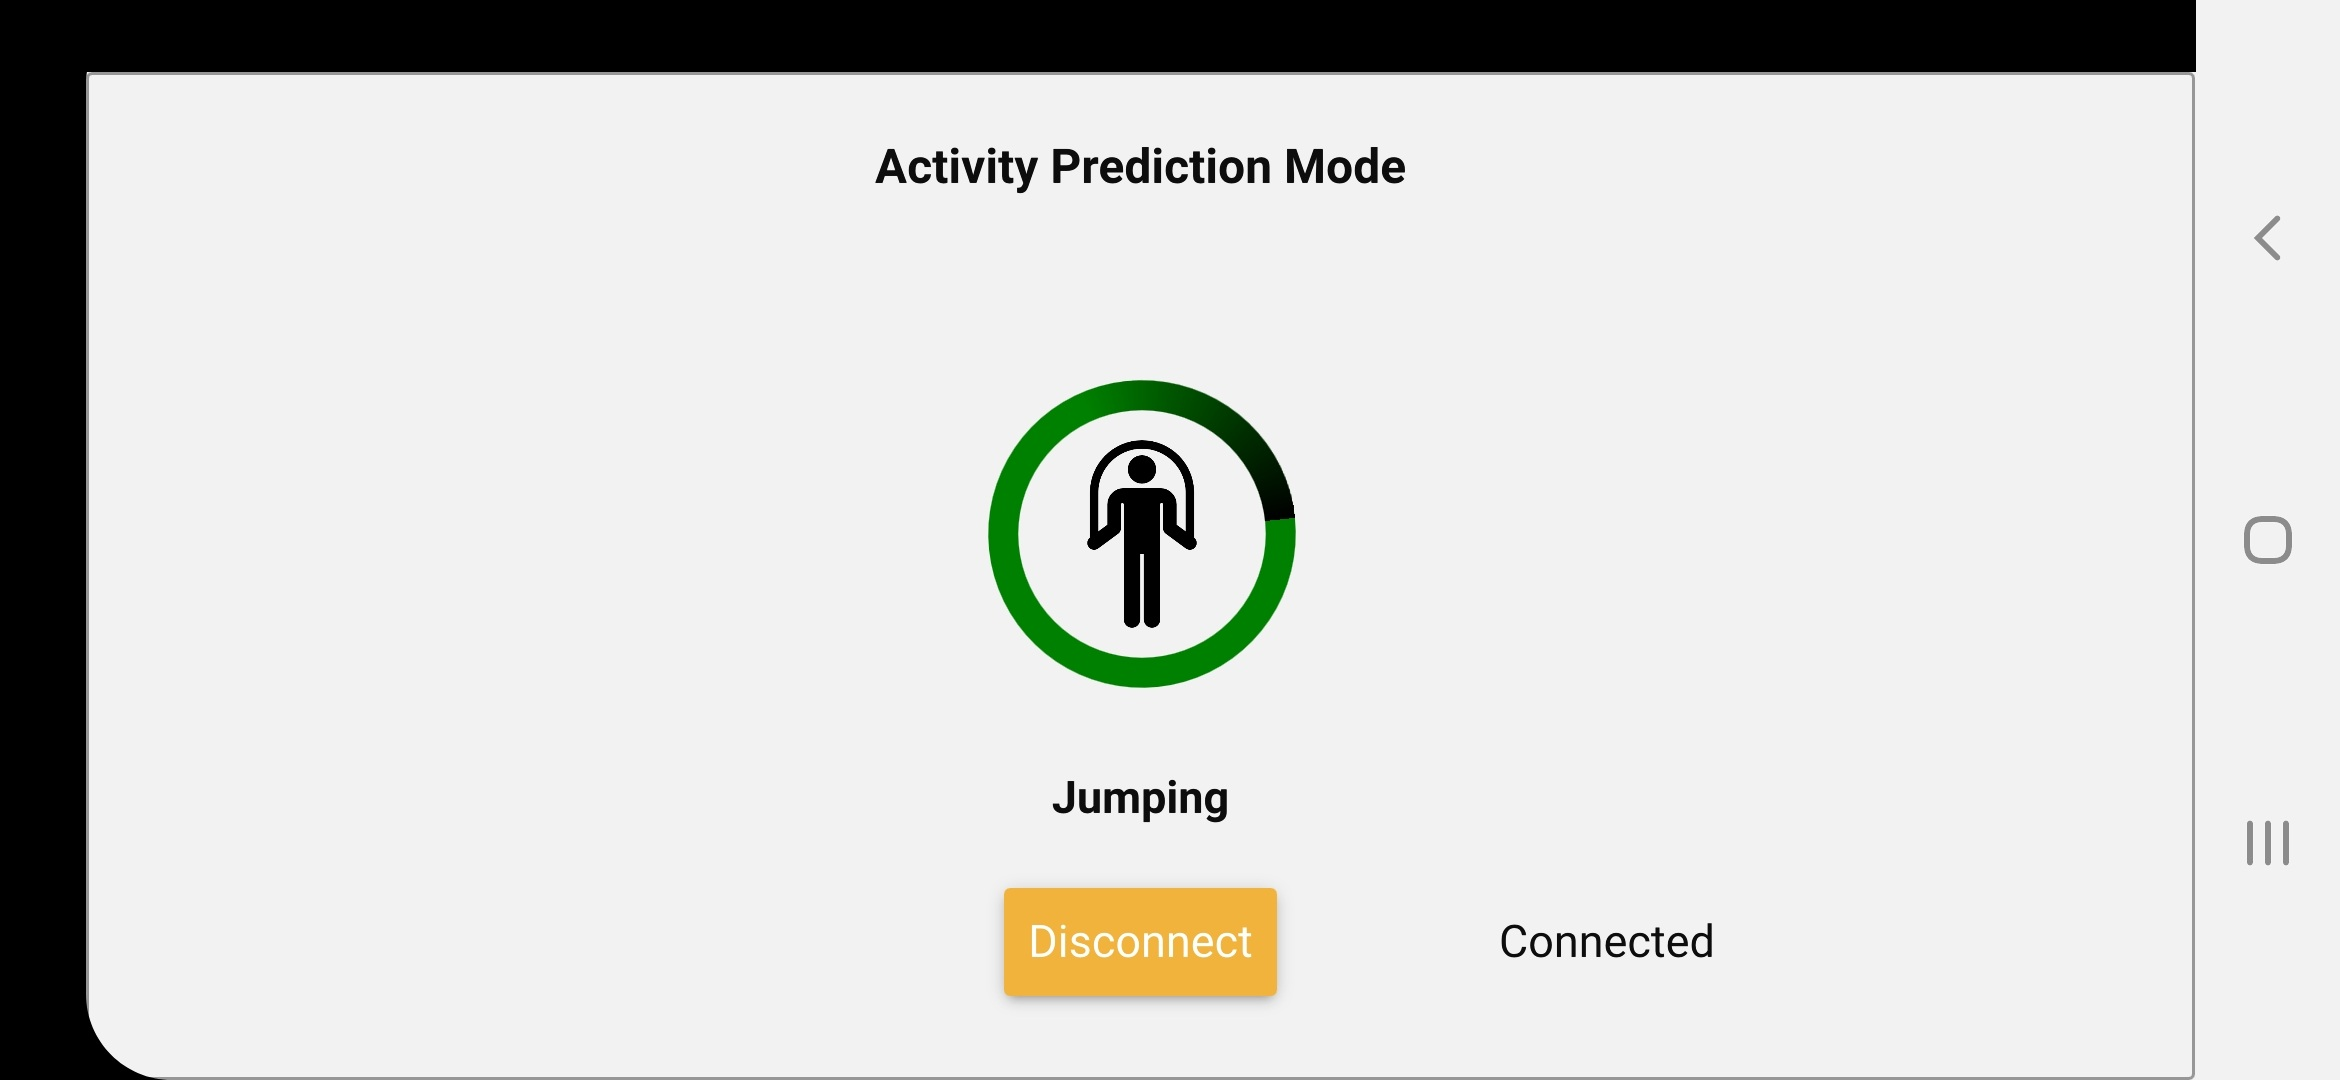
\includegraphics[width=0.4\linewidth]{./ImageFiles/jumping}
	%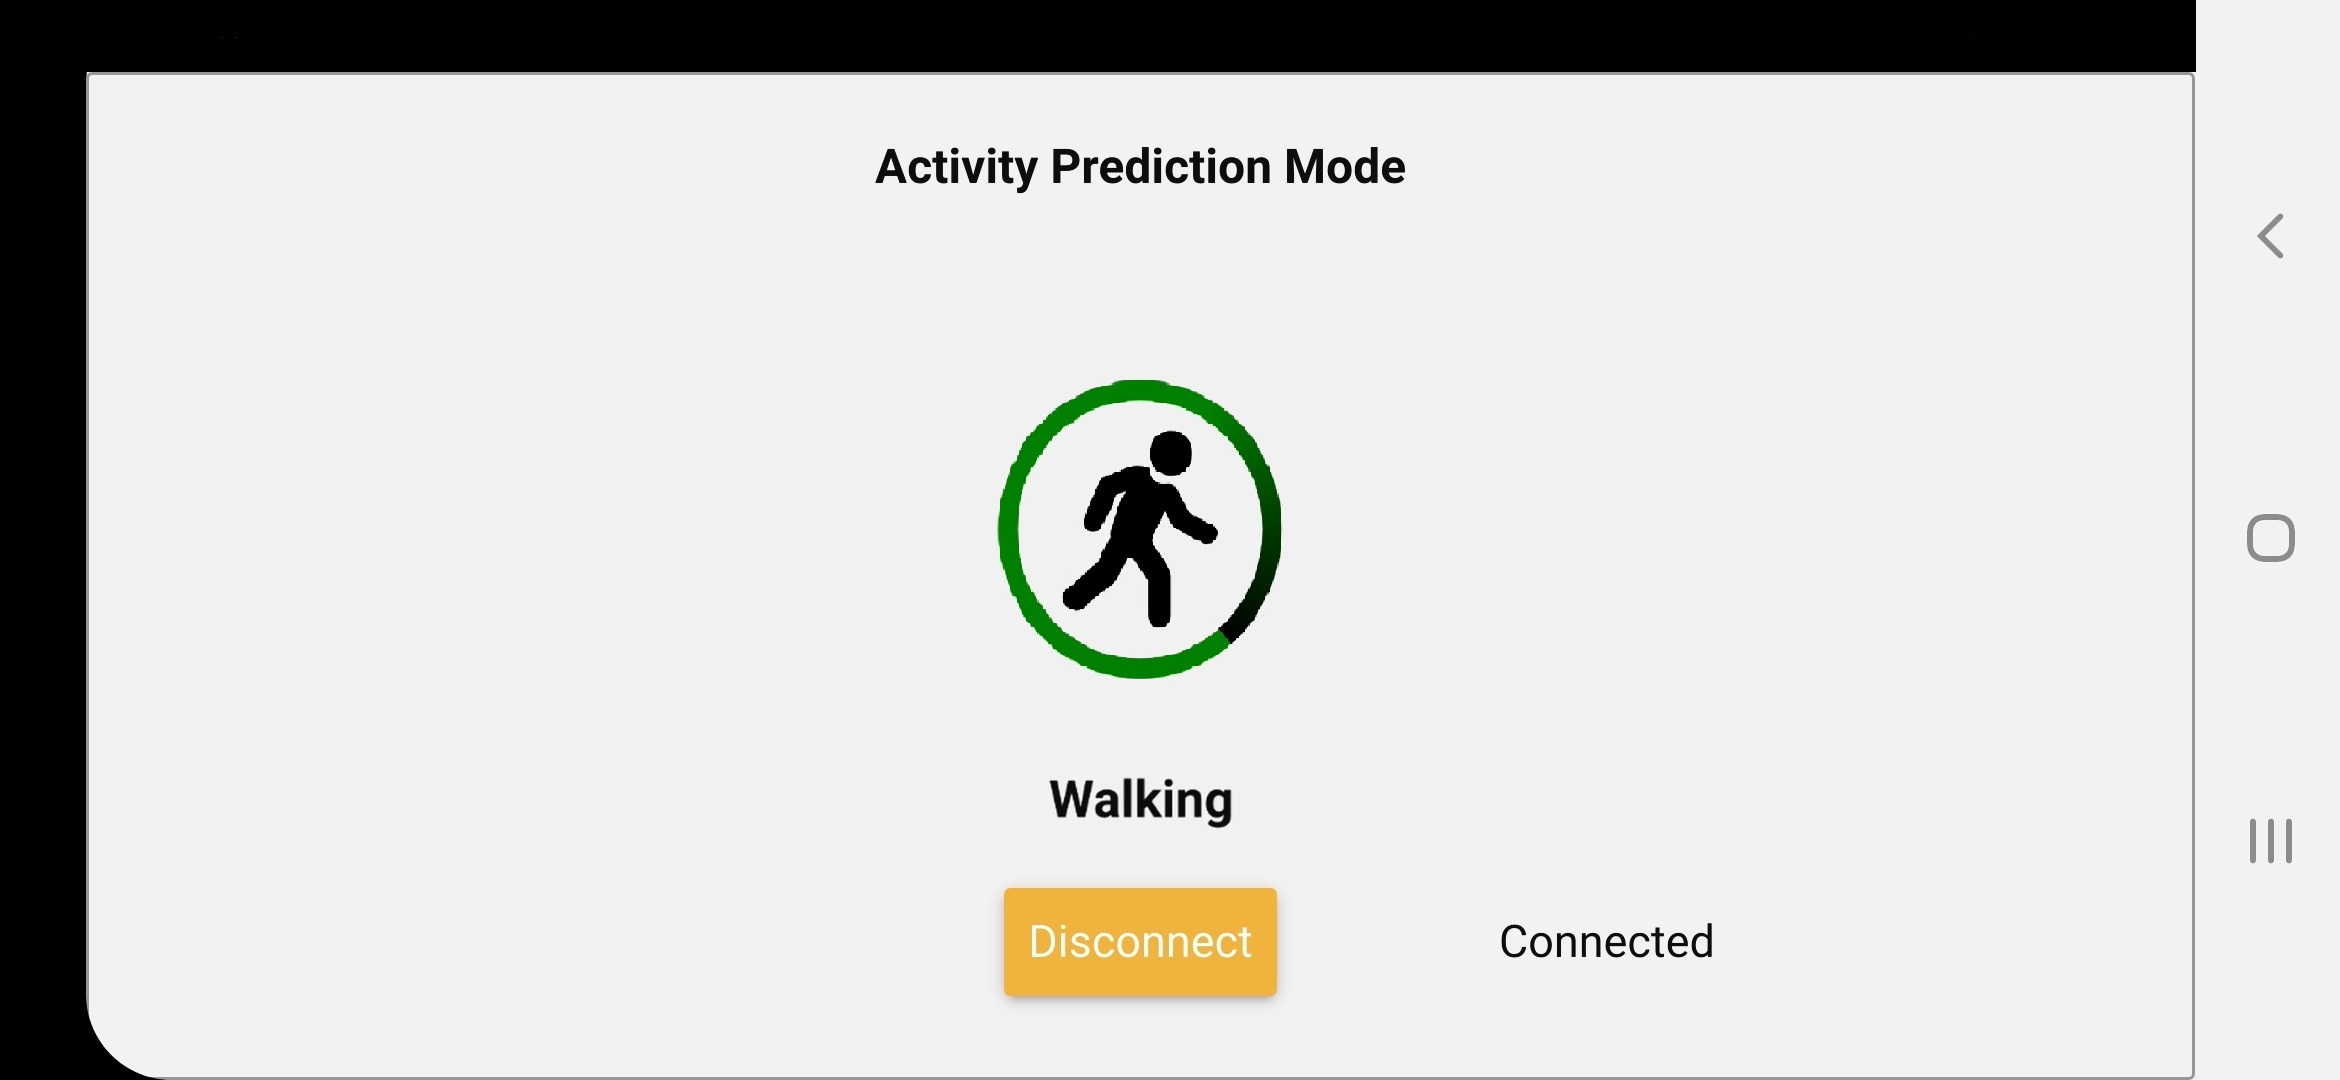
\includegraphics[width=0.4\linewidth]{./ImageFiles/walking}
	\caption{Schermate per le possibili attività: cyclette, fermo, salto della corda e camminata.}
	\label{fig:attivitafisica}
\end{figure}
\todo{manca schermata walking}
Invece nei momenti subito dopo la connessione del dispositivo al BLE oppure nei momenti in cui non si riesce a classificare l'attività in corso tra quelle possibili sull'applicazione viene visualizzata la schermata della figura \ref{fig:attivitaignota}.
\begin{figure}[tbh]
	\centering
	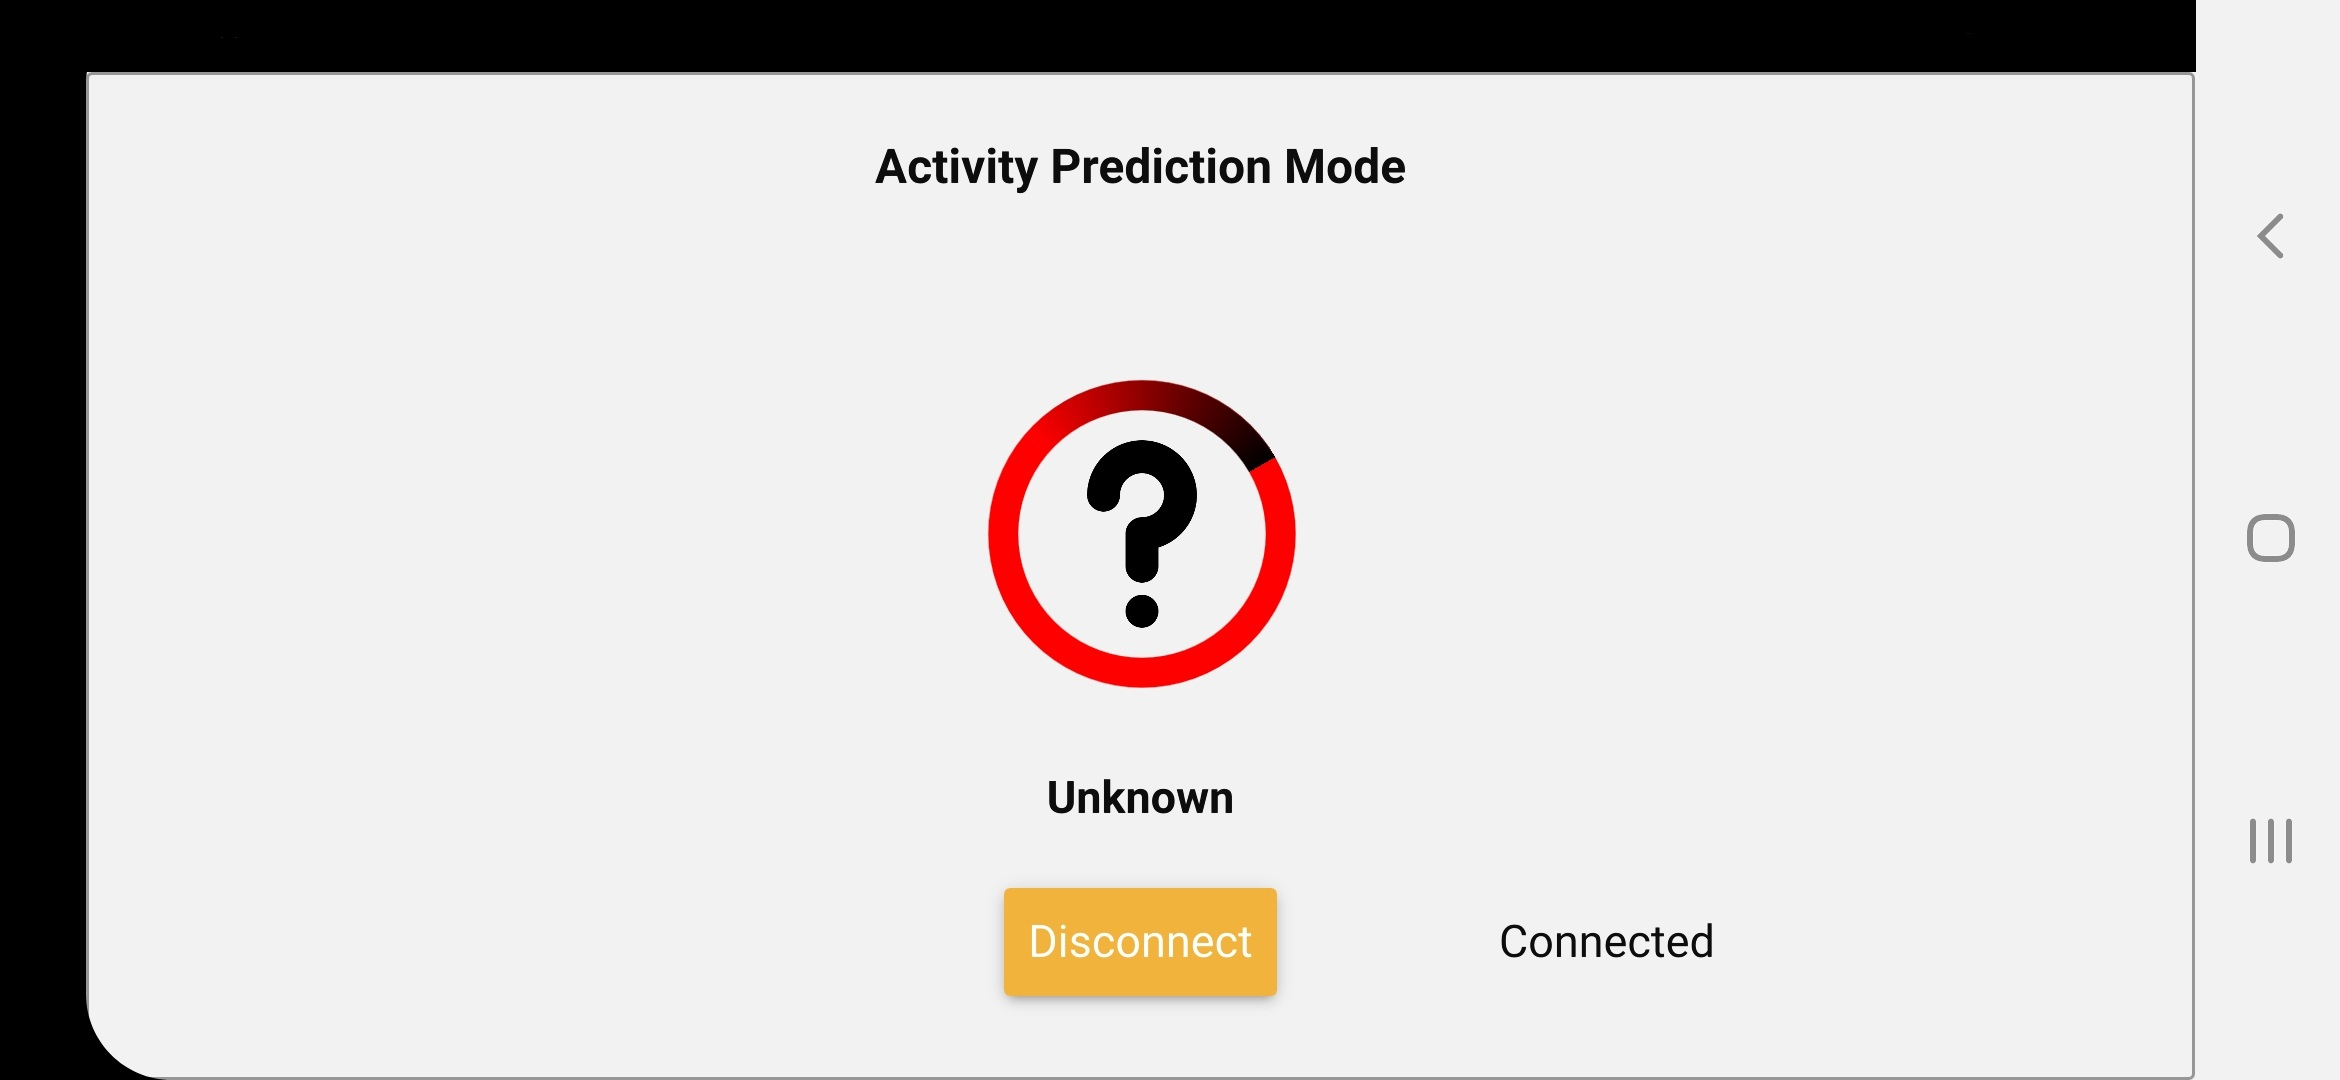
\includegraphics[width=0.4\linewidth]{./ImageFiles/unknown}
	\caption{Schermata per l'attesa iniziale dopo la connessione al BLE o per misure non classificabili.}
	\label{fig:attivitaignota}
\end{figure}

\subsection{Edge Impulse}
\todo{spiegazione framework, inserimento dati, suddivisione in training e test, foto dashboard, parametri di allenamento e risultati}
Edge Impulse è una piattaforma online per lo sviluppo di algoritmi di machine learning per edge devices. Tramite Edge Impulse è possibile creare un modello da poter caricare sul dispositivo finale seguendo quattro semplici passi: aqcuisizione dei dati, design del modello, test del modello e deploy del modello. 

Per prima cosa sono stati acquisiti i dati delle quattro categorie di attività fisica da classificare (idle, walking, jumping e cycling). Essendo un modello ML, maggiore è il numero dei dati, più preciso è il modello. I dati acquisiti sono stati poi caricati sulla piattaforma Edge Impulse. Come si può osservare in figura \ref{fig:acquisizione_dati}, è possibile dividere i dati in \textit{training set} e \textit{test set}: Edge Impulse suggerisce di dividere i dati di train e di test con una percentuale rispettivamente di 80\% e 20\%.
\begin{figure}[h!]
	\centering
	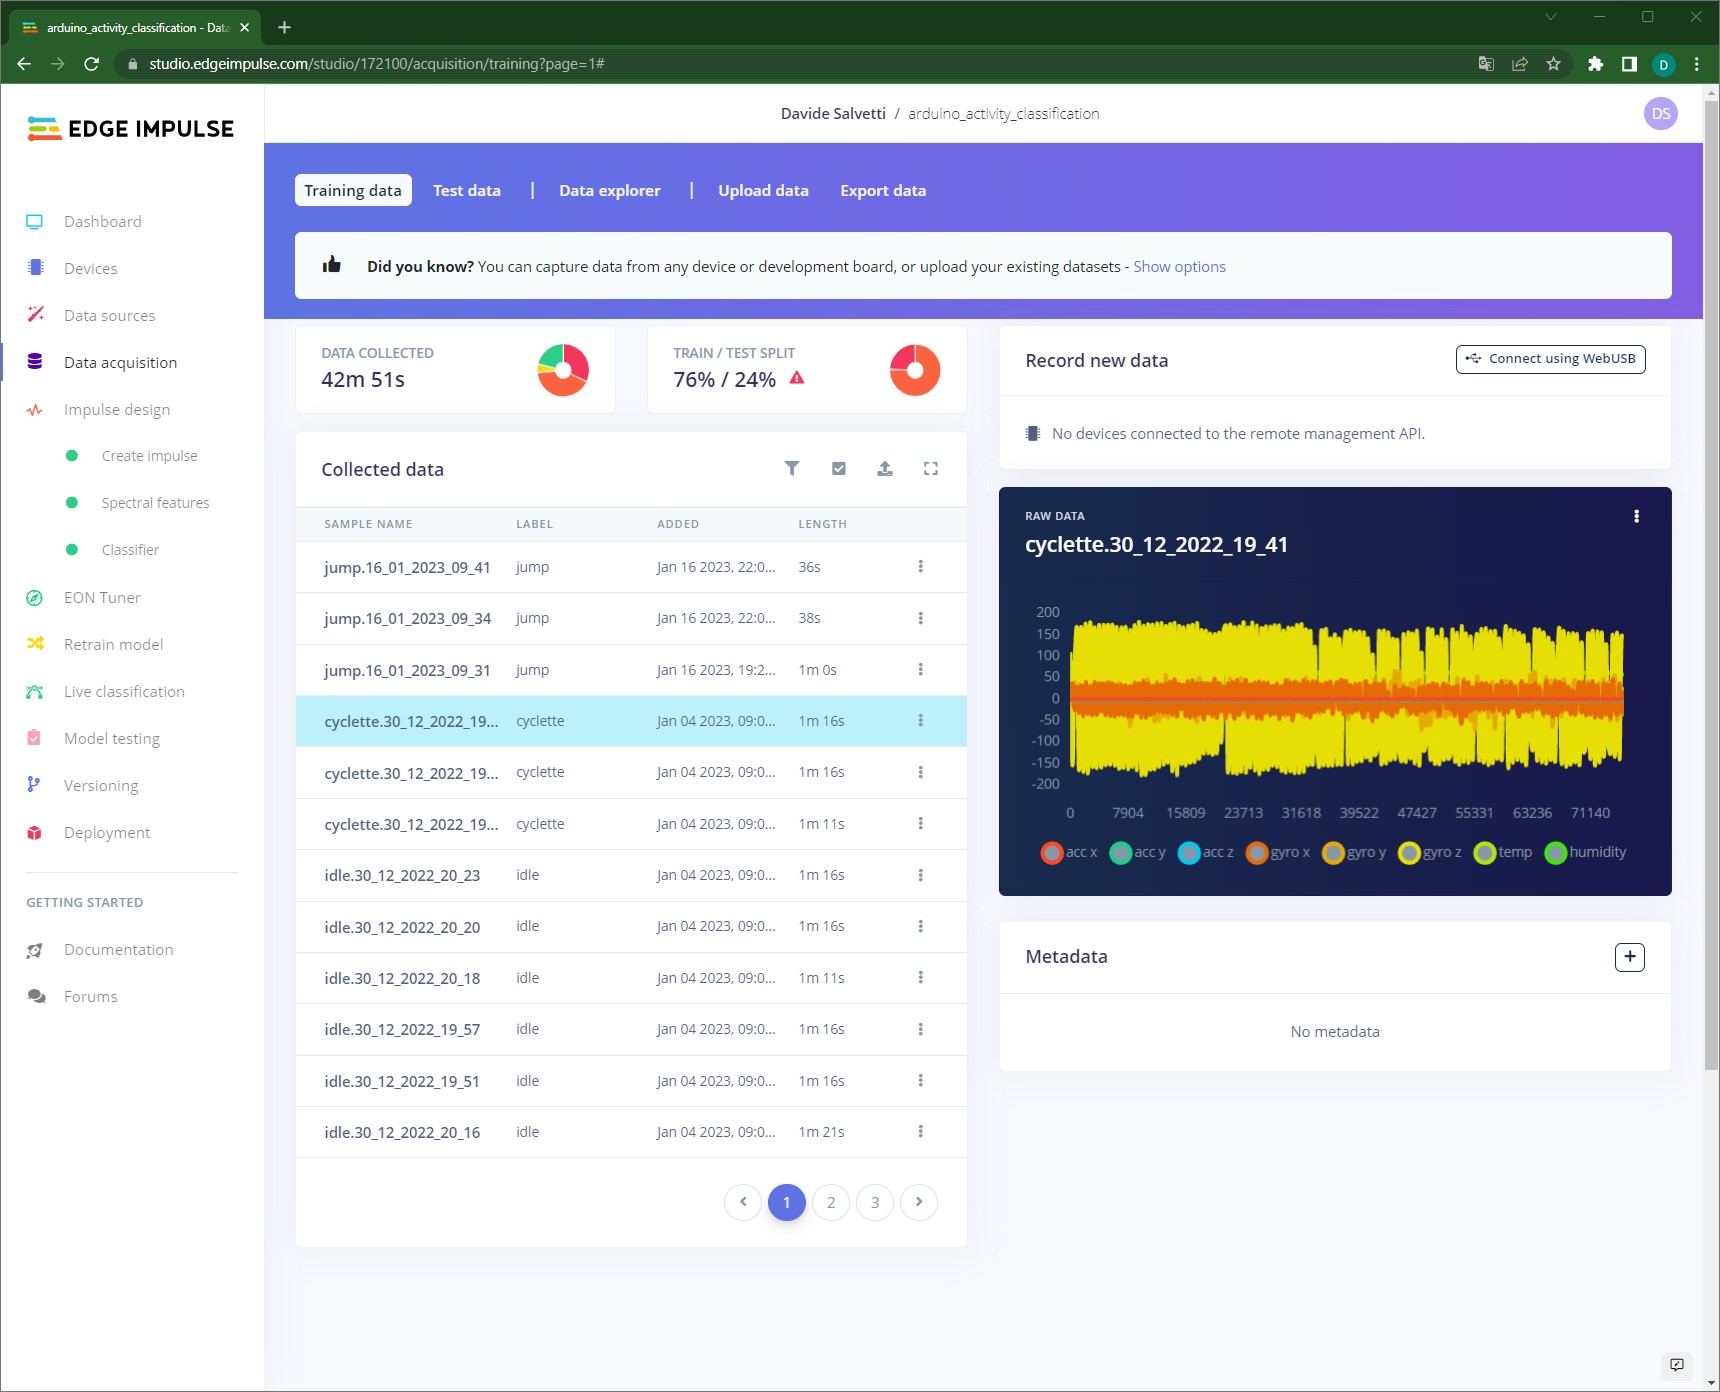
\includegraphics[width=0.5\linewidth]{./ImageFiles/data_acquisition.jpg}
	\caption{Schermata di Edge Impulse dove è possibile inserire nuovi campioni.}
	\label{fig:acquisizione_dati}
\end{figure}

Successivamente, è stato creato un \textit{impulse}: questa fase prevede la scelta delle finestre dei dati con relativa frequenza, di un blocco di processamento dei dati e di un blocco di learning (figura \ref{fig:creazione_impulse}).
\begin{figure}[h!]
	\centering
	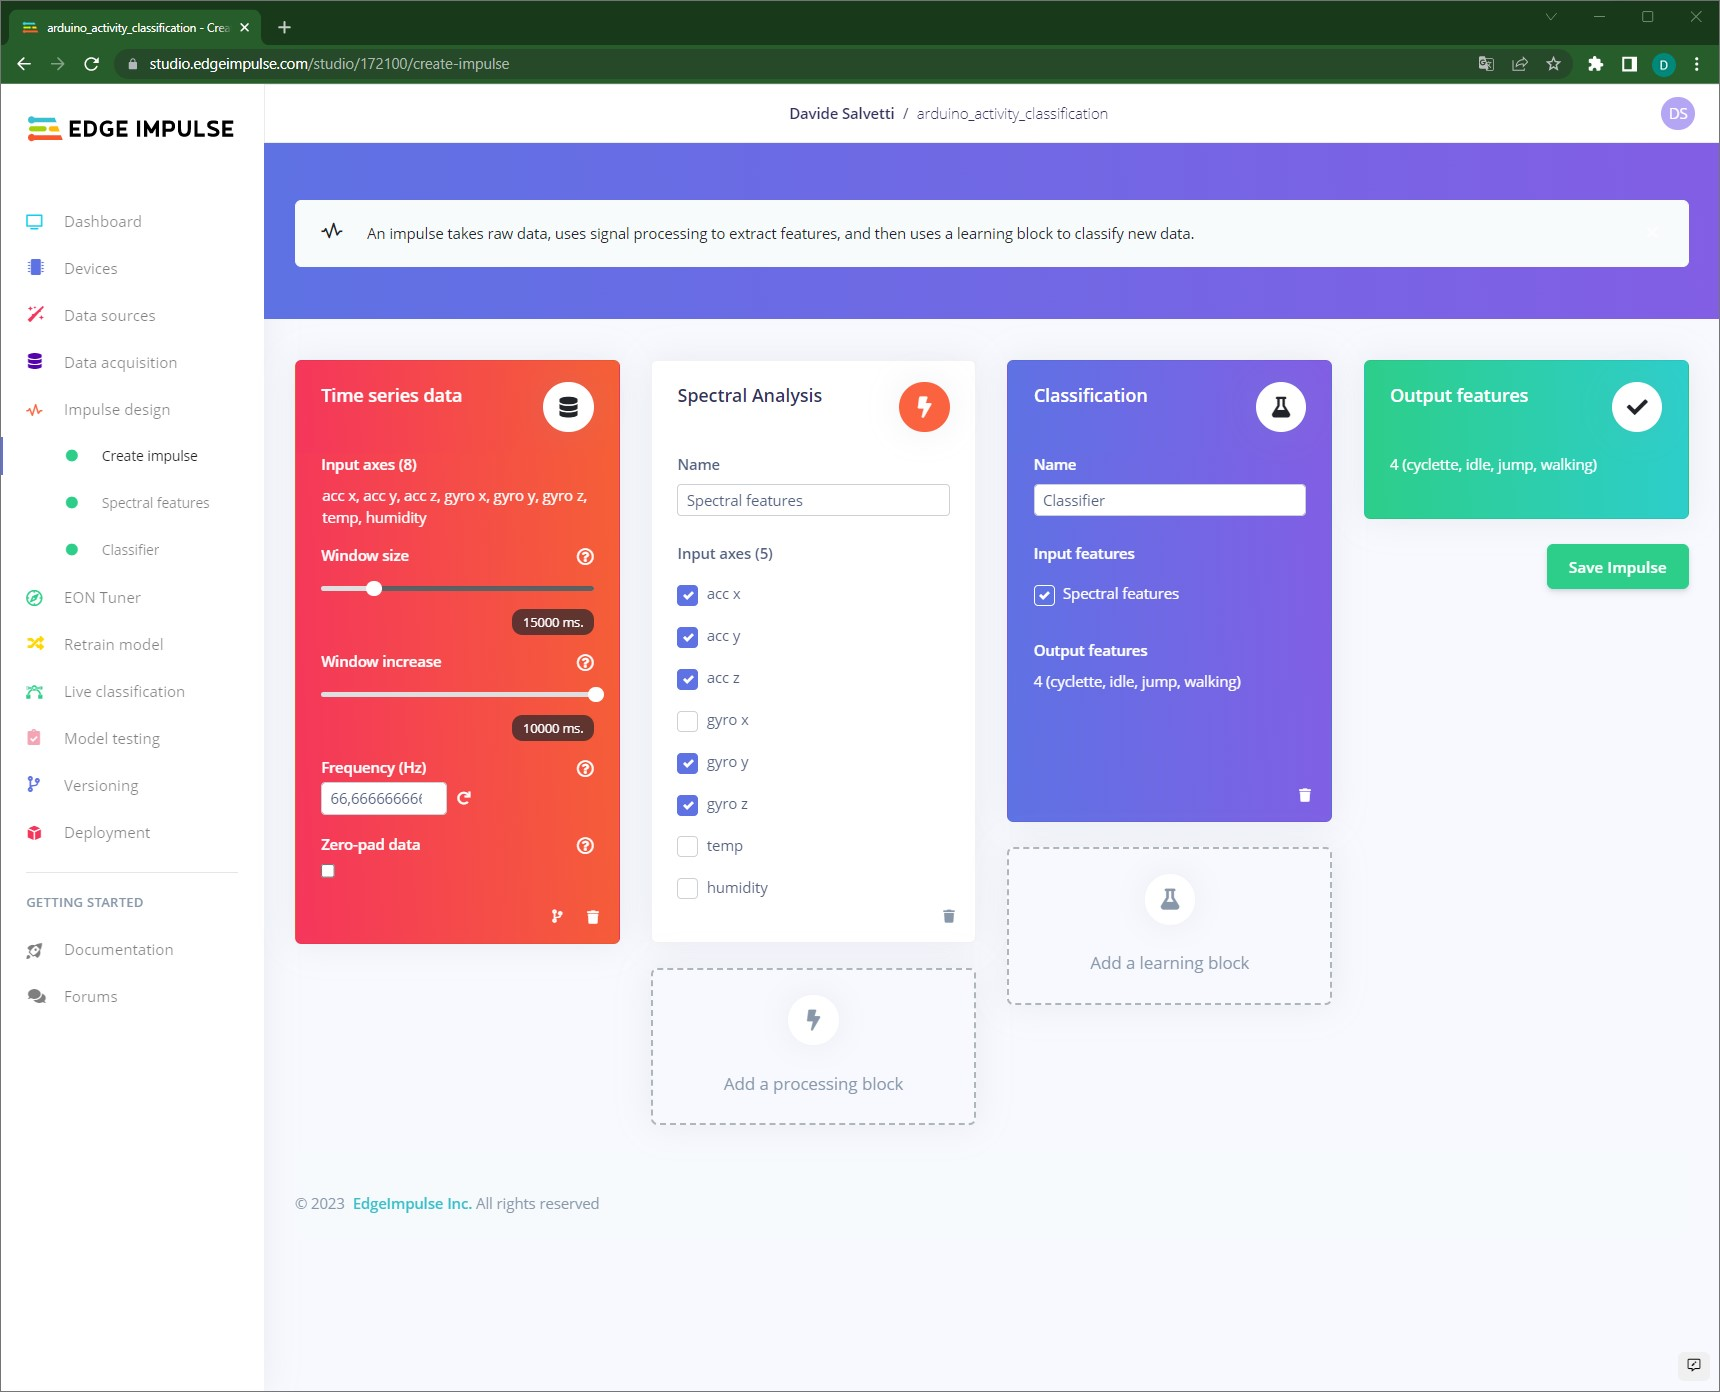
\includegraphics[width=0.5\linewidth]{./ImageFiles/creazione_impulse.jpg}
	\caption{Schermata di Edge Impulse per la creazione di un nuovo \textit{impulse} tramite la scelta di ciascun blocco.}
	\label{fig:creazione_impulse}
\end{figure}

I campioni vengono analizzati tramite finestre di 15 secondi con una slinding window di 10 secondi. La frequenza di campionamento viene ricavata a partire dai dati poichè in essi è presente il campo \texttt{timestamp}, ed è pari circa a \SI{66}{\hertz}.
Per il processamento dei dati è stato scelto un DSP che analizza le feature spettrali dei segnali provenienti da accelerometro e giroscopio. Come anticipato in precedenza, non sono stati inclusi i campi temperatura e umidità, ma nemmeno il giroscopio sull'asse x: infatti, osservando la figura \ref{fig:arduino_su_gamba}, si può notare che l'asse x è posizionato verticalmente e variazioni nel valore del giroscopio su tale asse si possono ricondurre a cambi di direzione durante il percorso che non sono significativi per la classificazione dell'attività\todo{per favore rileggere se ha senso, è un po complesso}.
Per l'analisi spettrale è stato scelto di introdurre un filtro passa-basso con frequenza di taglio a \SI{20}{\hertz} del sesto ordine ed è stato analizzato il logaritmo della densità spettrale di potenza (figura \ref{fig:spectral_feature}). Una volta definiti i parametri dell'analisi spettrale, il modello estrae le features dai dati di test e visualizza su un grafico i dataset divisi per somiglianza delle features; inoltre mostra l'importanza delle feature estratte per comparare le diverse classi: alcune delle feature più importanti sono il valore quadratico medio dell'accelerometro sull'asse x, la densità spettrale di potenza del giroscopio sull'asse z tra \SI{4.82}{\hertz} e \SI{5.08}{\hertz} e la densità spettrale di potenza dell'accelerometro sull'asse y tra \SI{4.56}{\hertz} e \SI{4.82}{\hertz} (figura \ref{fig:spectral_feature}).  

\begin{figure}[h!]
	\centering
	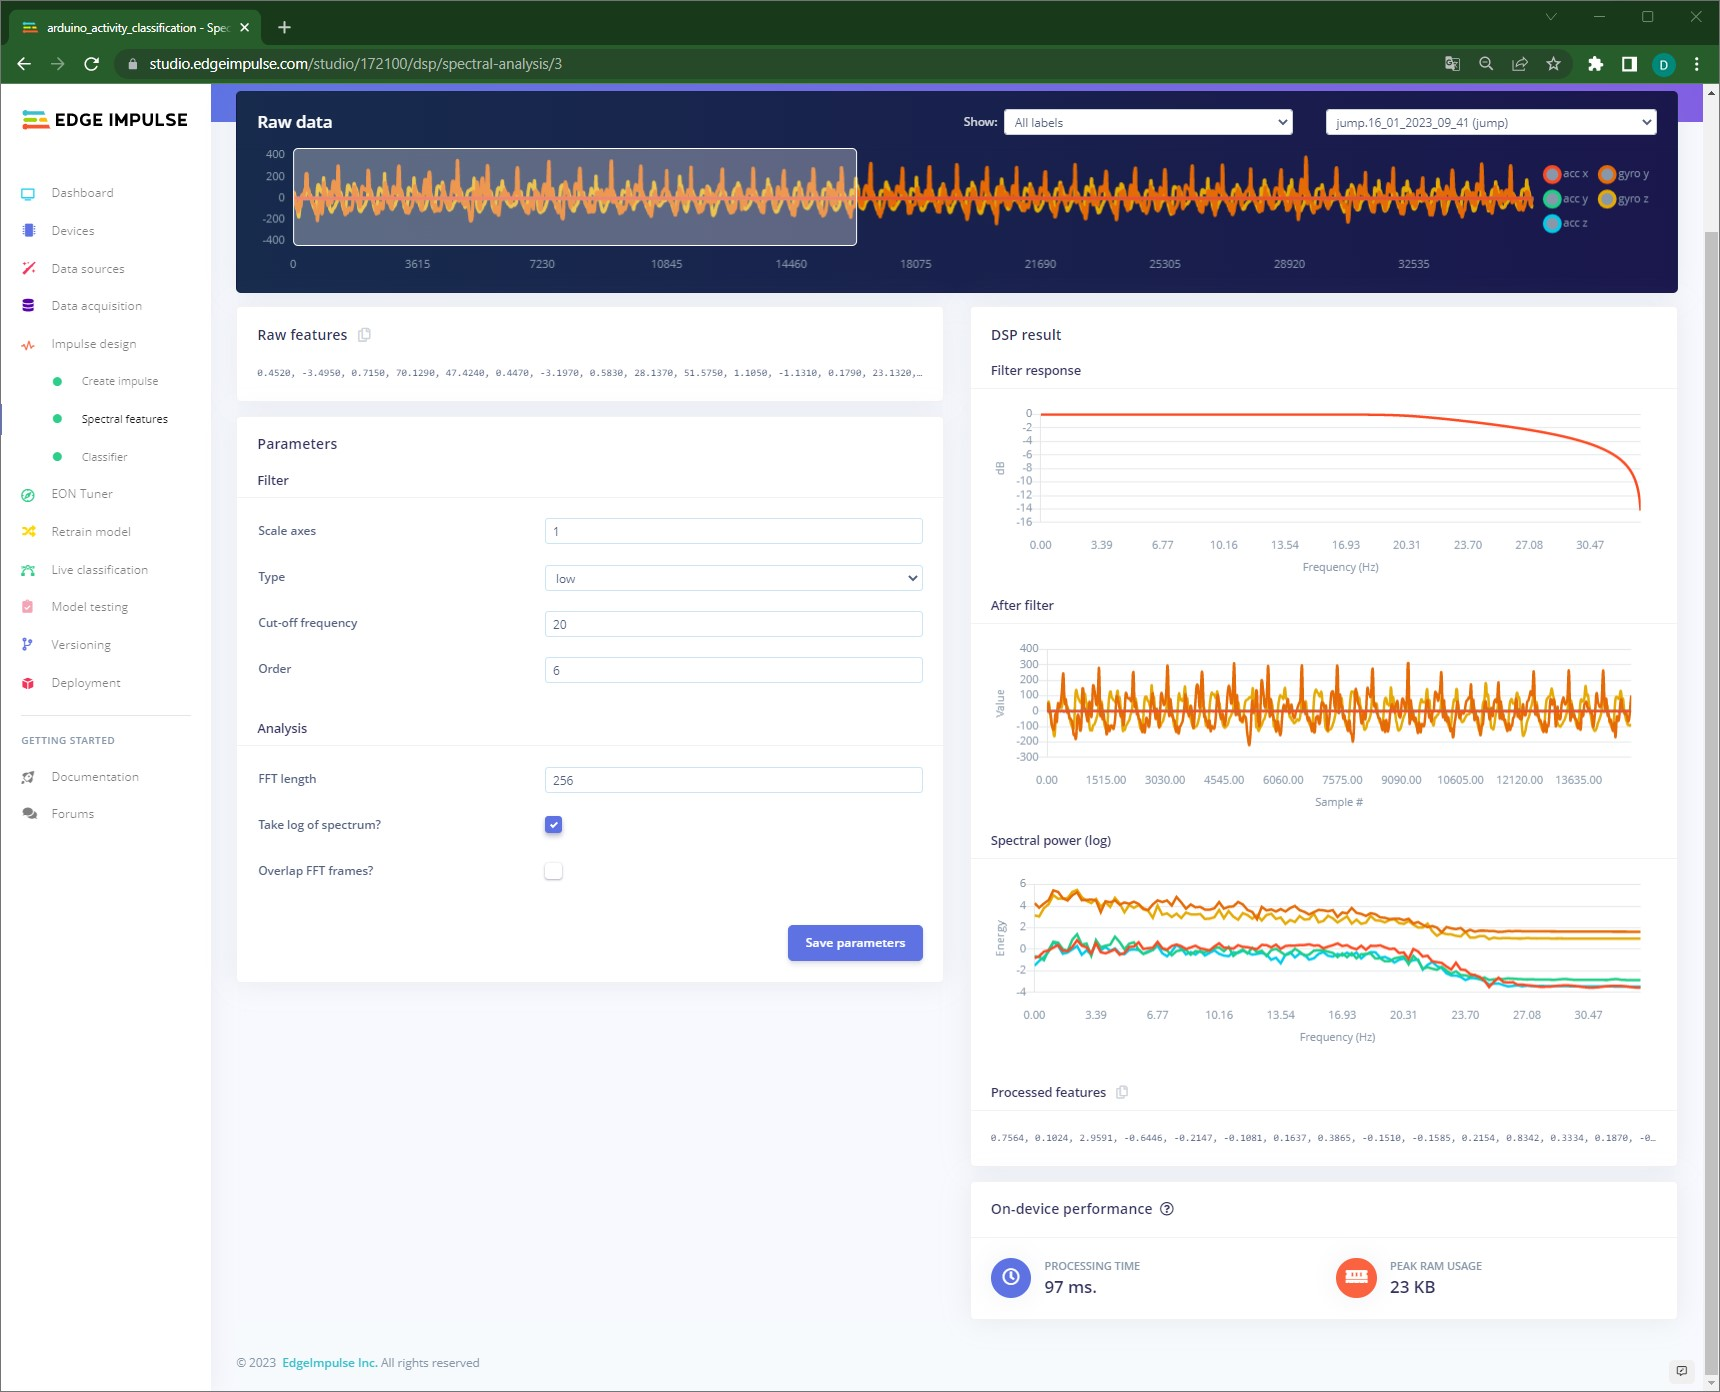
\includegraphics[width=0.49\linewidth]{./ImageFiles/spectral_features.jpg}
	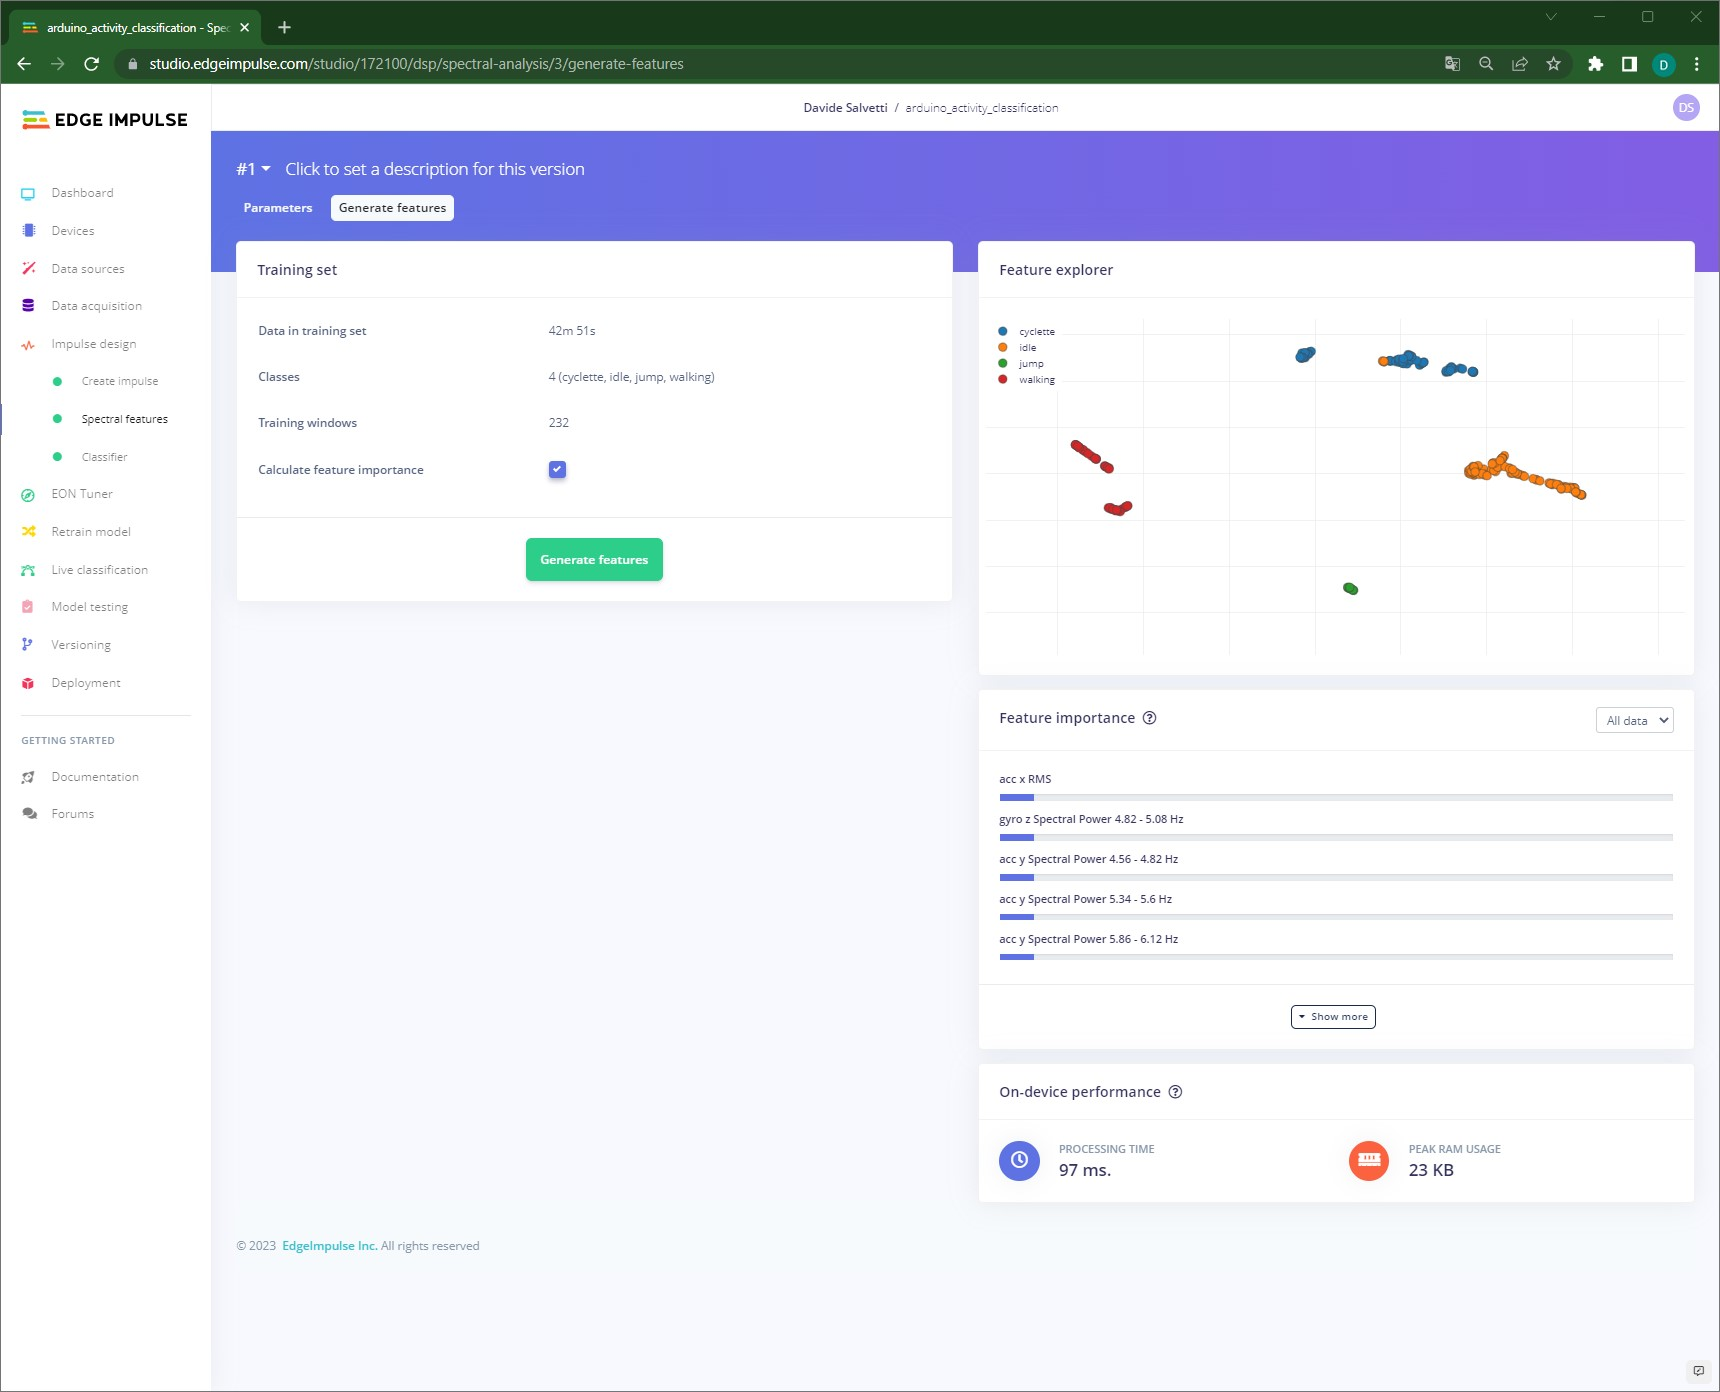
\includegraphics[width=0.49\linewidth]{./ImageFiles/features_extracted.jpg}
	\caption{A sinistra, schermata di Edge Impulse per il settaggio dei parametri per l'estrazione delle feature spettrali. A destra, schermata di Edge Impulse per la visualizzazione dell'importanza di ciascuna features estratta per la distinzione delle varie classi. Inoltre, è possibile osservare le performance stimate di tale analisi sull'Arduino.}
	\label{fig:spectral_feature}
\end{figure}

Come blocco di apprendimento è stato scelto un classificatore. La rete neurale riceve in ingresso 400 features ricavate dal blocco DSP precedente e le analiza tramite due Dense Layer, composti rispettivamente da 32 e 16 neuroni, ed un Output Layer che fornisce in uscita la probabilità di appartenenza delle feature in ingresso alle 4 classi. La predizione è la classe con probabilità maggiore. Anche in questo caso vengono mostrate le performance stimate del classificatore sul dispositivo in questione\todo{Qui ci sarebbe una immagine della matrice di confusione carina ma... dice hche l'accuratezza è del 100 per cento e non credo sia proprio corretto. Il problema credo sia sempre quello che i dati son solo miei e forse sono ancora pochi}. 

Una volta sviluppato il modello è possibile testarlo sui dati di test: in figura \ref{fig:model_test} è possibile osservare l'accuratezza del modello sui dati forniti, che è pari al 98.65\%. \todo{Bo, è alta l'accuratezza, sicuramente c'è un po di overfitting ma d'altronde son sempre tutti dati miei e non sono tantissimi. Magari scriviamolo.}

\begin{figure}[h!]
	\centering
	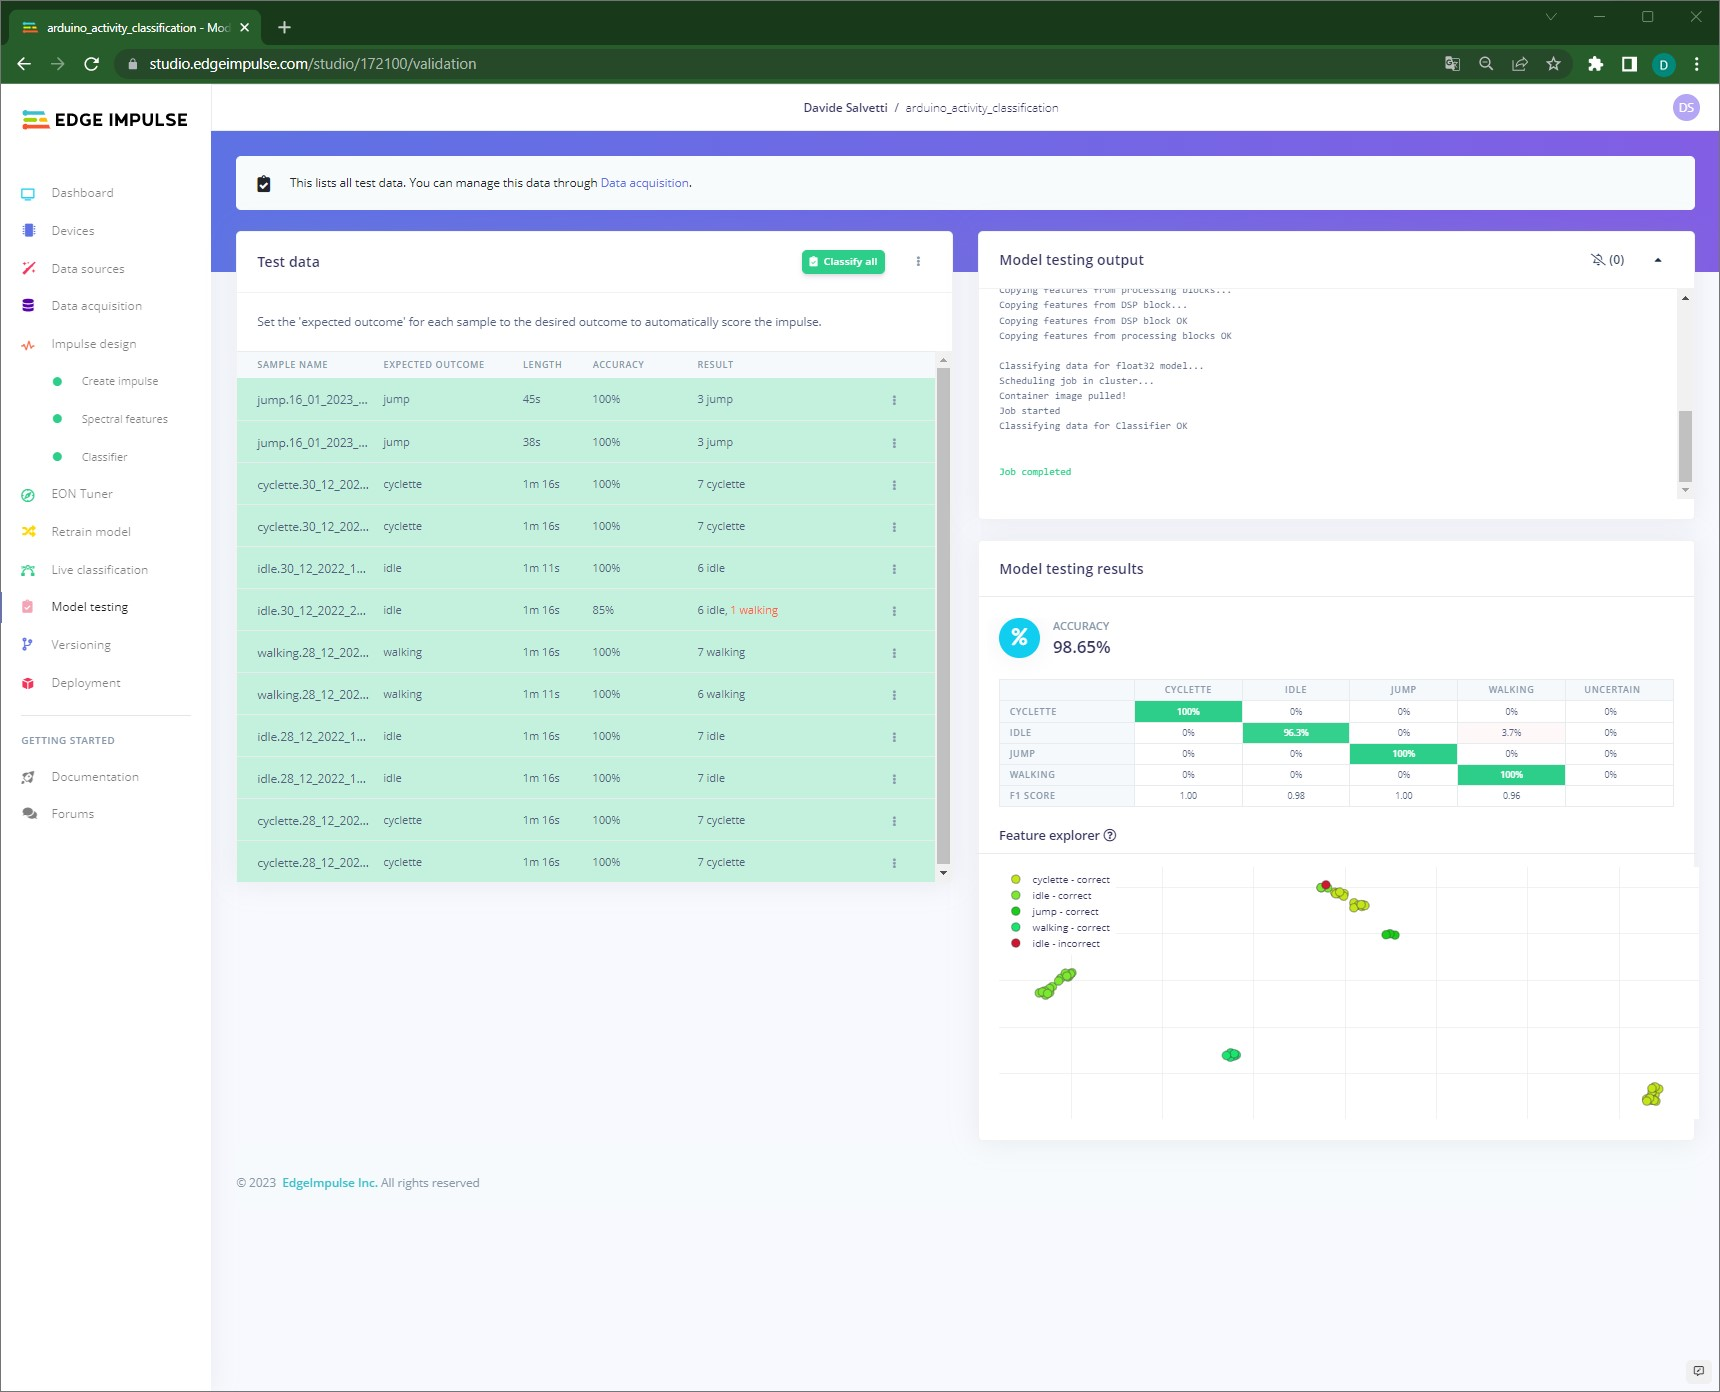
\includegraphics[width=0.5\linewidth]{./ImageFiles/model_test.jpg}
	\caption{Schermata di Edge Impulse per il testing dei dati che mostra l'accuratezza del modello.}
	\label{fig:model_test}
\end{figure}

La fase finale è quella di deploy. Il modello sviluppato, comprensivo del blocco DSP per l'estrazione delle features, può essere scaricato dalla piattaforma Edge Impulse come una libreria di Arduino, la quale può essere caricata direttamente sulla board. 


\subsection{Arduino} \label{arduinoSect}
 \todo{ottimizzazione del codice con buffer circolare (forse)}
Come preannunciato nella sezione \ref{classifSect}, il firmware per la classificazione è strutturato in 3 thread. Il loro funzionamento è rappresentato con la macchina a stati della figura \ref{fig:SM_classif}).
\begin{figure}[tbh]
	\centering
	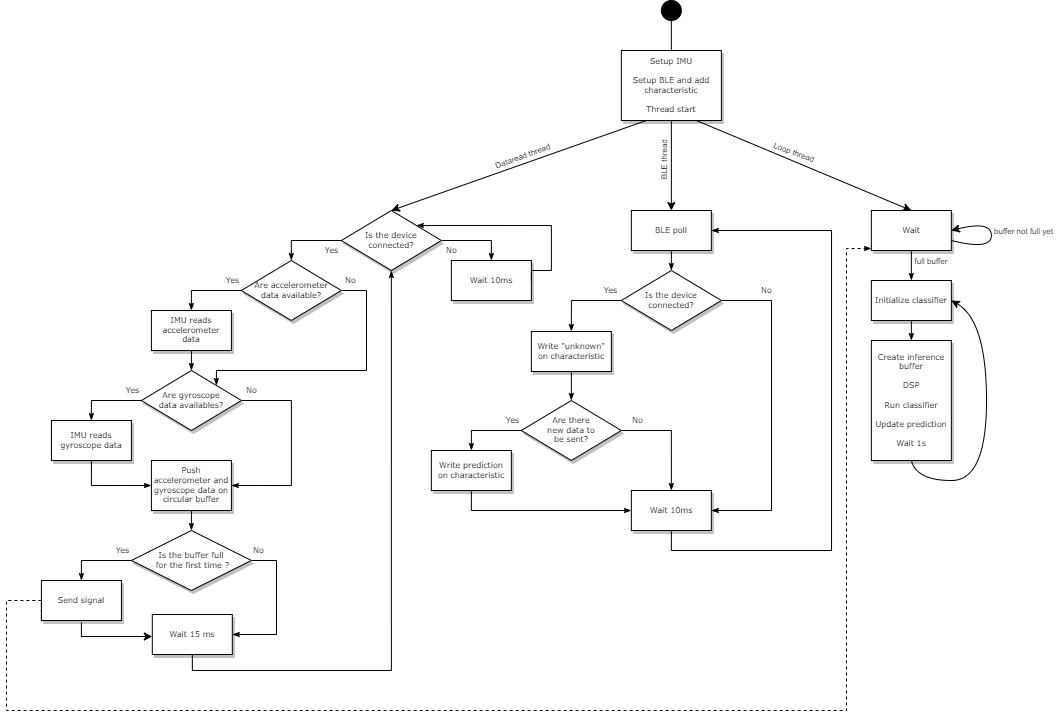
\includegraphics[width=0.8\linewidth]{./ImageFiles/SM_classification}
	\caption{Macchina a stati del firmware di classificazione dei dati sensoriali.}
	\label{fig:SM_classif}
\end{figure}
Nel Loop thread, la chiamata al classificatore corrisponde all'utilizzo delle librerie di Edge Impulse. Questa chiamata richiede come parametri in input il segnale, la variabile in cui salvare la previsione e un parametro che caratterizza l'inferenza.
\todo{integrazione libreria da Edge Impulse}
Per quanto riguarda i tempi di classificazione, il tempo necessario per passare da una classificazione alla successiva e quindi per cambiare la previsione è di circa 40-45 secondi. Questo tempo è dovuto al fatto che si deve svuotare il buffer e che si deve identificare per 6 volte la stessa attività prima di specificarla come previsione.